%!TEX program = pdflalatex
\documentclass[a4paper]{article}

\usepackage{PQS2016}

% \usepackage{graphicx}
% \usepackage{amssymb,amsmath,bm}
% \usepackage{textcomp}
% \def\vec#1{\ensuremath{\bm{{#1}}}}
% \def\mat#1{\vec{#1}}

\usepackage{ifluatex}
\ifluatex
  \usepackage{fontspec}
  \usepackage{polyglossia} % babel replacement for use with fontspec
  \setdefaultlanguage[variant=american]{english}
  \selectlanguage[variant=american]{english}
\else
  \usepackage[utf8]{inputenc}
  \usepackage[T1]{fontenc}
  \usepackage[american]{babel}
\fi

\usepackage[acronym, nomain, nowarn]{glossaries}
\loadglsentries{acronyms}
\usepackage{csquotes}
\usepackage{booktabs}
\usepackage[hyphens]{url}
\usepackage[pdfhighlight=/O, hidelinks, unicode=true]{hyperref}
\usepackage{amssymb}
\usepackage{mathtools}
\usepackage{fixmath}
\usepackage{algorithm2e}
\usepackage{subcaption}
\usepackage[load-configurations={abbreviations,binary}, per-mode=symbol,range-phrase = {\text{~to~}}]{siunitx}
\sisetup{load-configurations = abbreviations,binary-units}
\usepackage{tabu}
\makeglossaries
\usepackage[url=false,doi=false,backend=biber,style=ieee,isbn=false,sorting=none,minnames=1,maxnames=6]{biblatex}
\addbibresource{literature.bib}
\usepackage[inline]{enumitem}

\usepackage[np]{numprint}

\npstyleenglish

\sloppy % better line breaks
\ninept

\title{A Comprehensive End-to-End Lag Model for Online and Cloud Video Gaming}

\makeatletter
\def\name#1{\gdef\@name{#1\\}}
\makeatother
\name{{\em Firstname1 Lastname1$^1$, Firstname2 Lastname2$^2$, Firstname3 Lastname3$^1$,}}

\address{$^1$Chair of Modeling of Adaptive Systems, University of Duisburg-Essen\\
  $^2$UoV \\
  {\small \tt \{florian.metzger,tobias.hossfeld\}@uni-due.de, albert.rafetseder@univie.ac.at}
}

%
\begin{document}



\maketitle

\section*{Hello}

%!TEX root = paper.tex
%%%%%%%%%%%%%%%%%%%%%%%%%%%%%%%%%%%%%%%%%%%%%%%%%%%%%%%%%%%%%%%%%%%%%%%%%%%%%%%%
\begin{abstract}

Recently, online and cloud video games have been shifting into the 
focus of consumer and academic interest. 
%Online and cloud gaming might 
%be the next-big-thing after HTTP adaptive video streaming for the 
%fields of computer network performance evaluation and \acrshort{QoE} 
%modeling it. A quickly growing number of publications concerns itself 
%with assessing the subjective quality of those two game types. 
However, 
due to the nature of video games and their large diversity, assessments 
of subjective game quality  
are always specific to a single game, and arguably even specific to the 
exact experiment conditions, and are difficult to
transfer to any other game, even if they seem to be similar on the 
surface.

This paper aims to rectify this by providing a model for an underlying 
mechanic that is a governing property of most of such earlier results: 
The end-to-end lag of video games. The paper describes in detail the 
components of this lag model, and additionally provides a 
parametrizable simulation that calculates the lag.

Open Access Notice: The authors explicitly encourage the review and 
reuse of all the data and custom tools used in the preparation of 
this paper. The materials are available from the authors' public 
repository \cite{mas-ude-github}. 

% The online interactions and resulting user experience of the online 
%interaction of video games have been a topic of several publications in 
%the past. This trend was reinforced through the development of Cloud 
%Gaming with its strong dependence on good network conditions. Many of 
%these studies focus on subjective user assessments, as this is usually 
%an approach that quickly results in usable scores without going too 
%deep into technical details of video games. Contrary, objective and 
%\acrshort{QoS}-centric measurements are often much harder to conduct.

% This paper aims to offer some insights and best practices for the 
%realization of such objective online video game measurements. To 
%facilitate this, we first discuss two properties intrinsic to video 
%games which distinguish them from pure video streaming:
% \begin{enumerate*} 
% 	\item the framerate and 
% 	\item the game tickrate 
% \end{enumerate*}
% and their impact on the game's interactivity and end-to-end lag. 
%Derived from these properties three distinct measurement approaches and 
%their limitations are presented.

\end{abstract}

%!TEX root = paper.tex
%%%%%%%%%%%%%%%%%%%%%%%%%%%%%%%%%%%%%%%%%%%%%%%%%%%%%%%%%%%%%%%%%%%%%%%%%%%%%%%%
\section{Introduction}
\label{sec:introduction}

Recently, video games have garnered research interest from both the computer networking and the \gls{QoE} communities, focusing on network-related properties and the resulting \acrshort{QoS} and \gls{QoE} of individual video games. 
% Many of these research efforts were triggered through the contrivance of cloud gaming, though the user experience of online games still remains a topic of investigation and research. 
A quickly growing number of publications also concern themselves with assessing the \gls{QoE} of such games. These assessments are usually conducted through user studies, and when set up correctly they can produce meaningful results. However, the inherent diversity of games and their accompanying gameplay mechanics make it difficult to transfer any of these results from one game to another. In contrast to passively consuming videos, games are highly interactive, making the setup of such studies much more difficult. Compared to plain video streaming, underlying properties of video games are also not straight-forward to observe from the outside. Yet, in order to conduct proper measurements, it is essential to understand them. This work aims critically questions from past gaming user studies and derive lessons learned them as well as to give insights into some of gaming's core properties. To further this, an \gls{E2E} lag model is introduced which represents the lag between a user input event and the display of the event's results on the screen. The model describes game lag on the basis of other intrinsic game factors, such as the framerate and tickrate. Initial results with this model confirm the influence of framerate and tickrate on the \gls{E2E} lag and therefore also on the game's subjective interaction quality. This means that these two parameters need to be tightly controlled in subjective quality assessment studies.

%!TEX root = paper.tex
%%%%%%%%%%%%%%%%%%%%%%%%%%%%%%%%%%%%%%%%%%%%%%%%%%%%%%%%%%%%%%%%%%%%%%%%%%%%%%%%
\section{Overview and Background}
\label{sec:background}

Before constructing an end-to-end lag model, we first introduce some terms 
and concepts in subsections \ref{subsec:game-model} through 
\ref{subsec:e2e-lag}. Then, subsection \ref{sec:measurementapproaches} 
presents various lag measurement techniques.


%%%%%%%%%%%%%%%%%%%%%%%%%%%%%%%%%%%%%%%%%%%%%%%%%%%%%%%%%%%%%%%%%%%%%%%%%%%%%%%%
\subsection{Basic Game Model}
\label{subsec:game-model}

\begin{figure}[!t]
\centering
\removelatexerror
\begin{algorithm}[H]
 \While{game running}{
  sample input\;
  update game state\;
  render screen\;
 }
\end{algorithm}
\caption{Basic model of a continuous main video game loop.}
\label{alg:gameloop1}
\end{figure}

At their core video games are essentially feedback-directed 
real-time simulators. Figure~\ref{alg:gameloop1} overviews a 
simplified simulation loop consisting of three parts.
The game reads player input, updates the game state, and renders 
new screen contents. This loop repeats as long as the game is running. 
While the three parts are interrelated, and every component provides 
some form of input to the next, they may still proceed at their own 
intrinsic paces. (For example, the state of the game world is updated 
even if the player character does not move.)
In this simplified model, we distinguish a generic process for player 
input, a tickrate that governs the frequency of game state updates, and 
a framerate determining how often the screen is updated every second.

Note that actual game implementations sometimes choose to update 
parts of the game state on different fixed frequencies. For example, 
a physics effect that does not influence gameplay directly could be 
updated at only half the tickrate. Also, the parameters of the player 
input process depend on the game genre and on the player action 
currently performed. Please refer to Table~\ref{tbl:tickrates} for 
exemplary rates of current games.

%Popular examples for the fixed tickrates of 
%game servers include \SI{64}{\hertz} or \SI{128}{\hertz} for 
%\textsc{Counter-Strike: Global Offensive}, \SI{20}{\hertz} for 
%\textsc{Minecraft}, or \SI{30}{\hertz} for \textsc{Dota 2}.


\begin{table}[!t]
\caption{Exemplary table of some competitive and popular video game tickrates that are either known, speculated upon, or derived by counting update and command messages. Data was collected from various reliable and unreliable source and should be taken as-is.}
\label{tbl:tickrates}
	\centering
	\begin{tabu}{X[0.45]|X}
		\toprule
		\textbf{Video Game} & \textbf{Tickrate} \\
		\midrule
		CS: GO & Configurable \SI{64}{\hertz}/\SI{128}{\hertz} \\ \midrule
		Battlefield 4 & \SI{30}{\hertz} (\SI{10}{\hertz} for state outside of close proximity to player). \SI{60}{\hertz}/\SI{120}{\hertz} implemented on test servers. \\ \midrule
		Minecraft & max. \SI{20}{\hertz} \\ \midrule
		League of Legends & \SI{30}{\hertz} (guessed) \\ \midrule
		Dota 2 & \SI{30}{\hertz} \\ \midrule
		StarCraft II & supposedly either \SI{16}{\hertz} or \SI{32}{\hertz} \\ \midrule
		Eve Online & \SI{1}{\hertz} \\ \midrule
%		Sports Game 1 & \\ \midrule
		Project Cars & \SI{600}{\hertz} (Physics) \SI{250}{\hertz} (Input) \\ %https://twitter.com/projectcarsgame/status/551340759858040833
		\bottomrule
	\end{tabu}
\end{table}


%%%%%%%%%%%%%%%%%%%%%%%%%%%%%%%%%%%%%%%%%%%%%%%%%%%%%%%%%%%%%%%%%%%%%%%%%%%%%%%%
\subsection{Game Architecture Flavors}
% TODO: needs a better word than types, more like architectures. Feedback welcome
% TODO: need to find a better word than game (delivery) flavors

We next discuss how different implementations of game architectures  
set the local/remote boundary. Consider first a \textit{single-player game}
as depicted in Fig.~\ref{fig:component-model-local}. All of the 
components run locally. However, we previously mentioned that the 
three parts of the main game loop each progress at individual paces. 
Therefore, one may conceptually form an \textit{online video game} (see 
Fig.~\ref{fig:component-model-online}) by separating server-side 
input and state management components out of the single-player 
architecture. Now, player state information is transmitted to the 
game server across the network, and likewise, state updates from 
the server transit the network until they reach the game client.
Furthermore, the game server can be the central, authoritative 
point of state synchronization for other connected clients.
It should be noted that for reasons of network and processing efficiency, 
player input events are usually batched, and sent to the server according 
to a specific \textit{command message rate}.

%\textit{Online video games} (i.e. mostly multiplayer games) complicate this update logic a bit as seen in the depiction of Fig~\ref{fig:component-model-online}. In client/server online games, the client is not the final authority over its game state any more. Instead, interpreted input commands are sent to the server and a preliminary game state is calculated locally. When the authoritative update from the server is received the two states can be once again be synchronized. 

Another possible separation of components is presented in 
Fig.~\ref{fig:component-model-cloud}: Now the game client, which includes 
state management and rendering, is situated on a remote entity. This gives rise to 
\textit{cloud gaming}, which is a form of \textit{game streaming} 
where the game streaming server is part of a larger streaming service 
hosted at a data center. Due to the spatial separation of the 
input/output devices and the game engine, input data needs to be 
sent from the streaming client to the game engine. The return channel 
does not transport game state messages in this scenario, but rather streams the 
rendered audio and video data.

Fig.~\ref{fig:tickrate-streamed} gives once again an overview of all these components for a combined streamed online video game scenario.

\begin{figure}[!t]
  \centering
  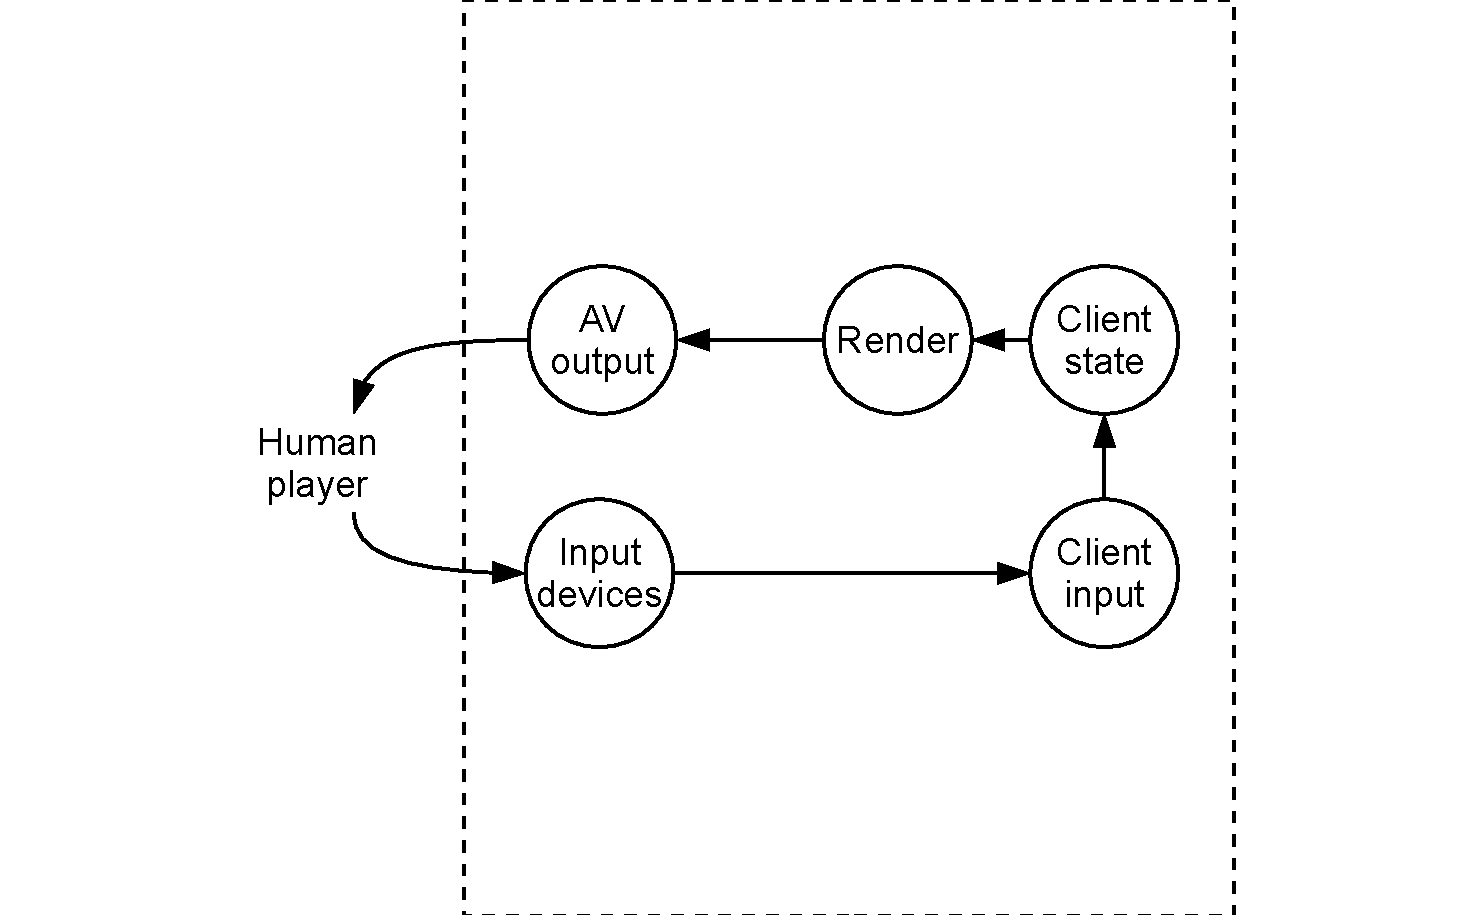
\includegraphics[width=0.8\columnwidth]{../models/component_interaction-local.pdf}
  \caption{Components and interactions of a singleplayer video game.}
  \label{fig:component-model-local}
\end{figure}

\begin{figure}[!t]
  \centering
  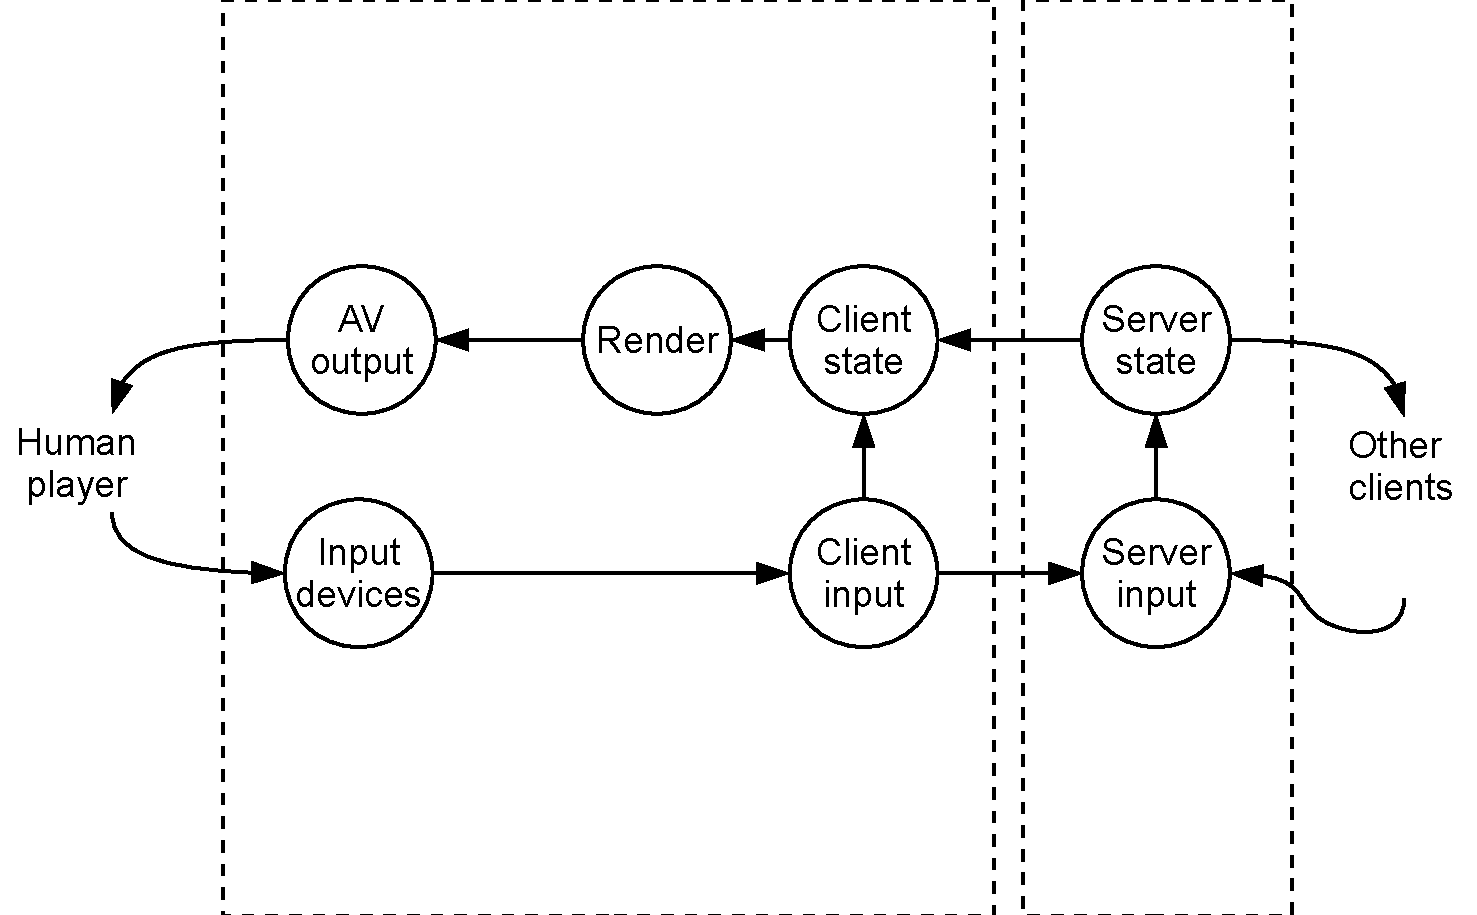
\includegraphics[width=0.8\columnwidth]{../models/component_interaction-online.pdf}
  \caption{Components and interactions of an online video game. Local game state is synchronized with the server's view on the game state.}
  \label{fig:component-model-online}
\end{figure}


\begin{figure}[!t]
  \centering
  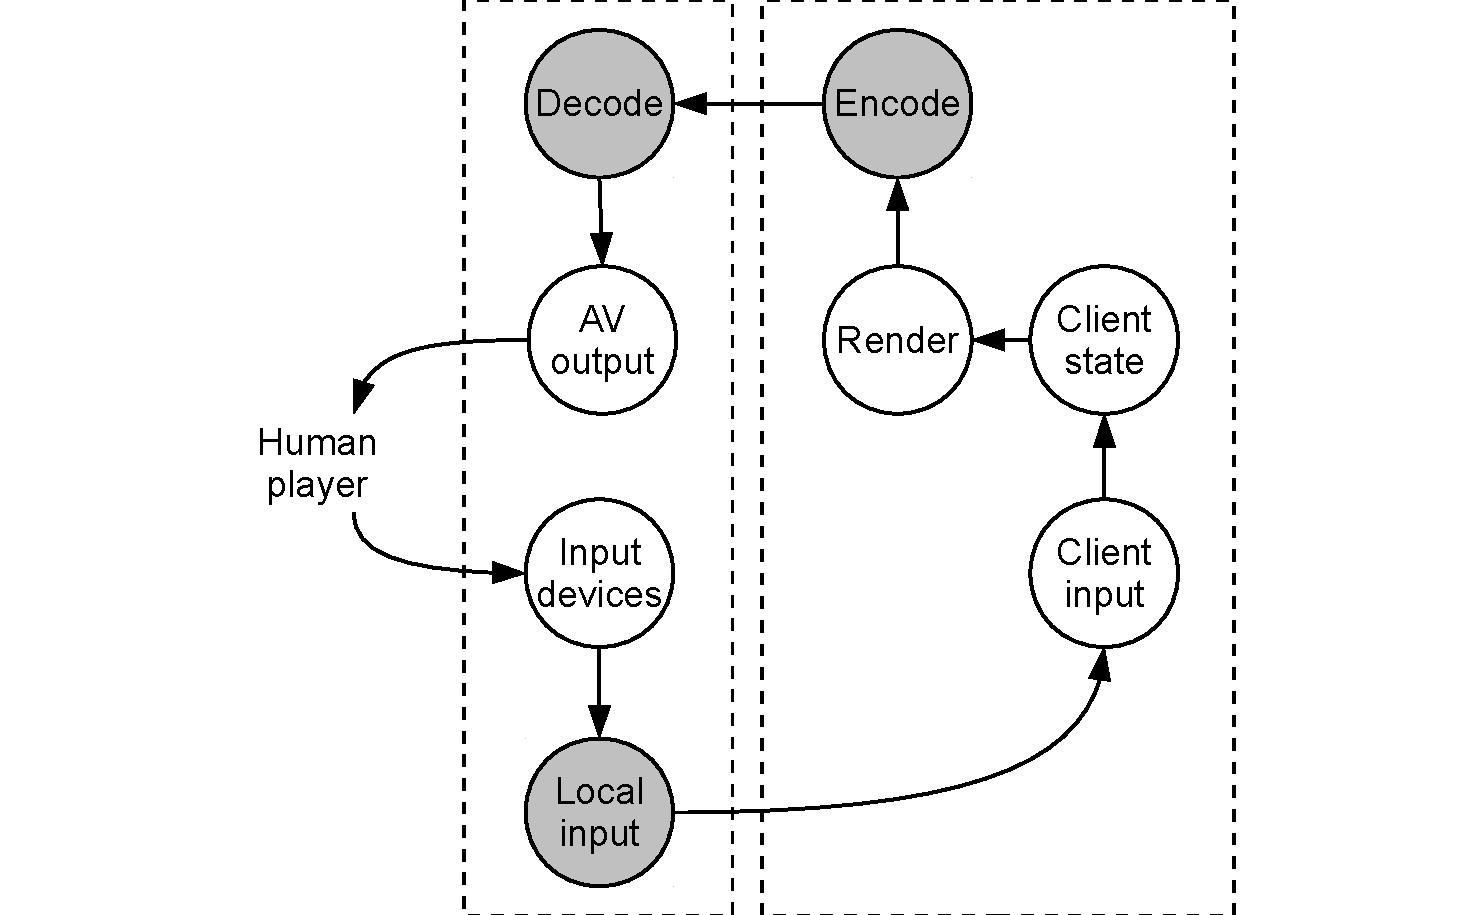
\includegraphics[width=0.8\columnwidth]{../models/component_interaction-cloud.pdf}
  \caption{Components and interactions of a streamed video game. I/O and game engine are physically separated and have to be synchronized.}
  \label{fig:component-model-cloud}
\end{figure}


\begin{figure}[!t]
	\centering
	\includegraphics[width=1.0\columnwidth]{../models/game-tick-rate-streamed.pdf}
	\caption{Interaction of client and server in streamed online games.}
\label{fig:tickrate-streamed}
\end{figure}


%%%%%%%%%%%%%%%%%%%%%%%%%%%%%%%%%%%%%%%%%%%%%%%%%%%%%%%%%%%%%%%%%%%%%%%%%%%%%%%%
\subsection{Framerate and Frame-times}
\label{sec:framerate}

In contrast to traditional video media with their fixed framerates of, e.g., \SI{24}{\hertz}, video games are more flexible but simultaneously also much more demanding to the framerate for several reasons. First, video games usually target frame rates of \SI{30}{\hertz}, \SI{60}{\hertz}, or sometimes also \SI{120}{\hertz}, depending on the type of game. Higher frame rates are targeted to enable smoother camera movement and scene transitions, as games often present faster scenes when compared to videos. High frame rates also help in increasing the interactivity as video games constantly require input on short time scales to which the game reacts and displays the feedback. Therefore, the framerate also influences the reactivity of a game, but can also be a source of latency itself.


%%%%%%%%%%%%%%%%%%%%%%%%%%%%%%%%%%%%%%%%%%%%%%%%%%%%%%%%%%%%%%%%%%%%%%%%%%%%%%%%
\subsection{End-to-End Lag}\label{subsec:e2e-lag}

Lag in video gaming is often described solely on the basis of the network delay in an online game. It should be evident that the lag is a critically important factor for almost all games. This is especially true for fast or competitive games, as it governs the reaction time to in-game events.

But this focus on network delay neglects some key components to this lag, including the input device, the time to sample and process the input, the game engine and server and their tickrates, frame rendering time, and ultimately the time to display the frame on the monitor. Only if all sources are factored in the complete \textbf{end-to-end lag} is captured. What makes matters even worse, is that this lag is usually not constant but can vary depending on the type of action triggered by the input. While some simple actions, say opening the menu, may have a very short lag, more complex interactions, e.g., issuing a move command, may take considerable longer to complete, partly due to the actions taking more than one game tick to complete. Therefore, each video game will have a distinct ``lag profile''.  


% TODO:
% This subsection adds the player to the architectures introduced above, highlights potential QoS and QoE (or discusses why some chosing a particular QoE metric is not useful) metrics to study. At the end of this section, the reader should agree that end to end latency is a sensible starting point to study video game qos.


%%%%%%%%%%%%%%%%%%%%%%%%%%%%%%%%%%%%%%%%%%%%%%%%%%%%%%%%%%%%%%%%%%%%%%%%%%%%%%%%
\subsection{Measurement Approaches}
\label{sec:measurementapproaches}

With the central role of the end-to-end lag in mind, it is natural to assume, that this lag also plays a critical role in both subjective and objective video game quality assessments. Therefore, the end-to-end lag needs to be correctly examined and quantified from any kind of video game. But video games usually represent a black box with very few points, where something can be actually measured. The following sections discuss three distinct methods which are each situated at an unique vantage point as depicted in Fig.~\ref{fig:measurement-methods}.

\begin{figure}[!t]
    \centering
    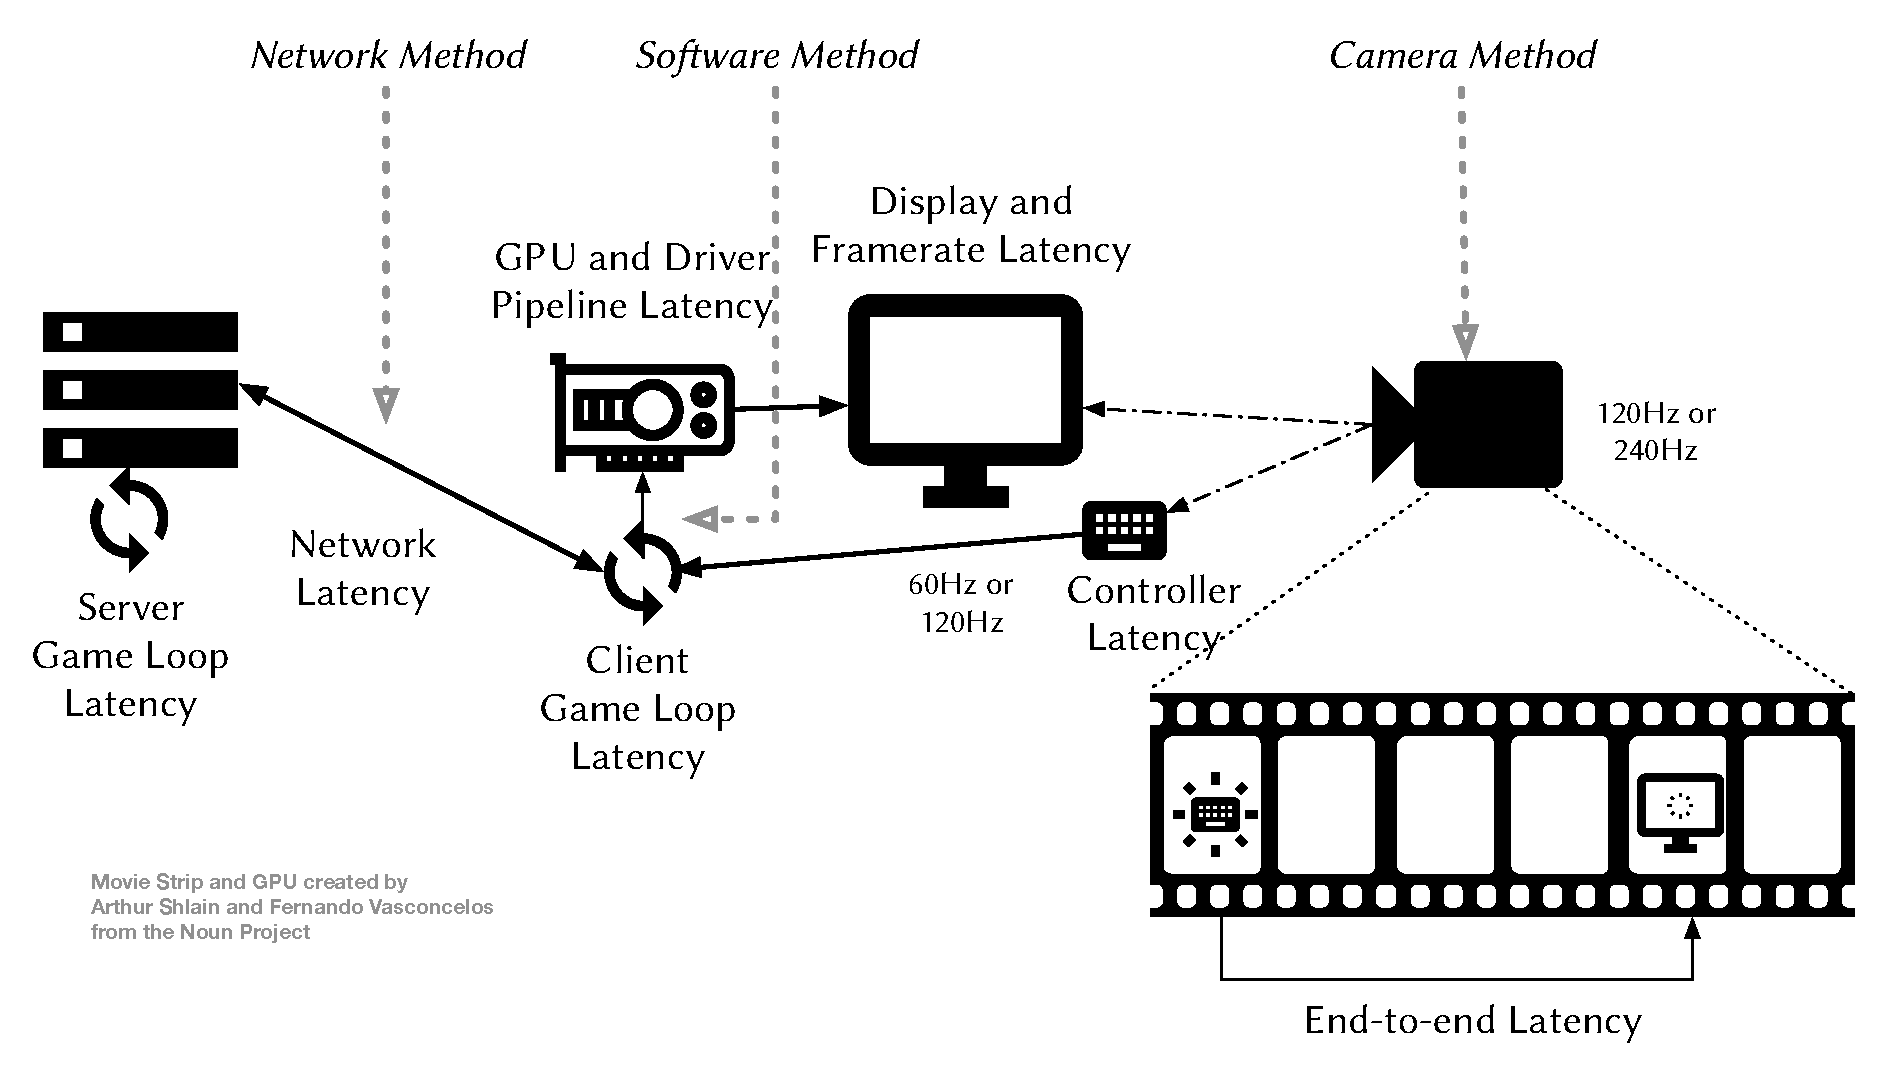
\includegraphics[width=1.0\columnwidth]{../models/e2e-lag.pdf}
    \caption{Location of the three measurement approaches to capture end-to-end latency inside a usual online video game lag chain.}
\label{fig:measurement-methods}
\end{figure}


%%%%%%%%%%%%%%%%%%%%%%%%%%%%%%%%%%%%%%%%%%%%%%%%%%%%%%%%%%%%%%%%%%%%%%%%%%%%%%%%
\paragraph{Screen Recording Software Method}
Recording the output stream of a video game might be the simplest approach to determine video game lag. It can capture both the framerate and \gls{IAT} at a driver level, and the recorded video can be used for image and quality analyses as well as to correlate it to additionally recorded input events in order to calculate the lag. This is not the complete end-to-end lag however, as both the controller and screen output delay are missing. The need to install additional software might make it unsuitable for some scenarios, e.g., when measuring console video games. As a variant of this method, one can also record the output stream with a video capture card on a secondary computer, which does not negatively effect the game's performance as the software method would.

Examples of this approach include both \cite{Chen:2011:MLC:2072298.2071991} and \cite{6670099} which measured the latency of cloud gaming services in the game client. They do this by invoking the system menu in games and measuring the time until it is displayed. A 2013 paper \cite{6574660} investigates the quality of cloud gaming interactiveness (i.e., the lag) as well as image quality by employing software recording methods on the client's computer.
%However, this method assumes a constant delay of game actions and may not capture the actual end-to-end lag of many of real game actions, as they are typically different from and longer as the latency of displaying a menu. A 2013 paper \cite{6574660} investigates the quality of cloud gaming interactiveness (latency) as well as image quality by employing software recording methods on the client's computer. With these techniques the challenges regarding the quality are discussed.


%%%%%%%%%%%%%%%%%%%%%%%%%%%%%%%%%%%%%%%%%%%%%%%%%%%%%%%%%%%%%%%%%%%%%%%%%%%%%%%%
\paragraph{Passive Network Measurements}
In some cases it may also be advantageous to tap into the network interactions of the games and record the command and update messages sent between server and clients. While this is not a direct measure of game quality, it can give insights into the game's inner workings, such as the tick rates, and one can derive, e.g., the lowest achievable end-to-end lag from this.

%Can only investigate command and update messages, not tick rate directly. Evaluate rate, IAT, and bandwidth, estimate latency (though there may be no direct link between commands and updates).

% Besides simple flow-based or packet-counting network metrics, many games also allow for deeper packet-dissecting analyses, as the often rely on standardized protocols or data formats, such as Protobuf\footnote{\url{https://developers.google.com/protocol-buffers/}} or incorporate well-known third-party multiplayer-enabling libraries. %And cloud games sometimes use derivates from the RTP-family or XMPP-based(VERIFY) protocols. 
% Additionally, almost no game encrypts its time-critical messages, enabling an easy read-out. Through these means, the specific commands can be read from the network and potentially linked to their effect on the game state in the corresponding state update messages.
%, but also potentially allowing malicious actions to be taken easily.


%%%%%%%%%%%%%%%%%%%%%%%%%%%%%%%%%%%%%%%%%%%%%%%%%%%%%%%%%%%%%%%%%%%%%%%%%%%%%%%%
\paragraph{Camera Recordings}
Finally, the only method to fully capture the end-to-end lag is to simultaneously record both the screen and input device through an external camera. The experimenter then has to count the frames between pressing a button on the input device and the action appearing on the screen and calculate the lag from this. For better visibility the input device is usually modified with an LED that turns on when the button is pressed. Also, the camera should operate at least at twice the monitor's refresh rate according to the Nyquist-Shannon sampling theorem. An additional benefit of this method is, that the game and the computers remain unaltered and are therefore not affecting any properties of the game. A variant of this approach, replacing the camera with a photodiode and synthetically creating the input events with a microcontroller is described in \cite{beyermethod}, though it may be difficult to use for certain game actions that have a barely visible or unpredictable on-screen effect.




% \begin{figure}
%   \centering
%   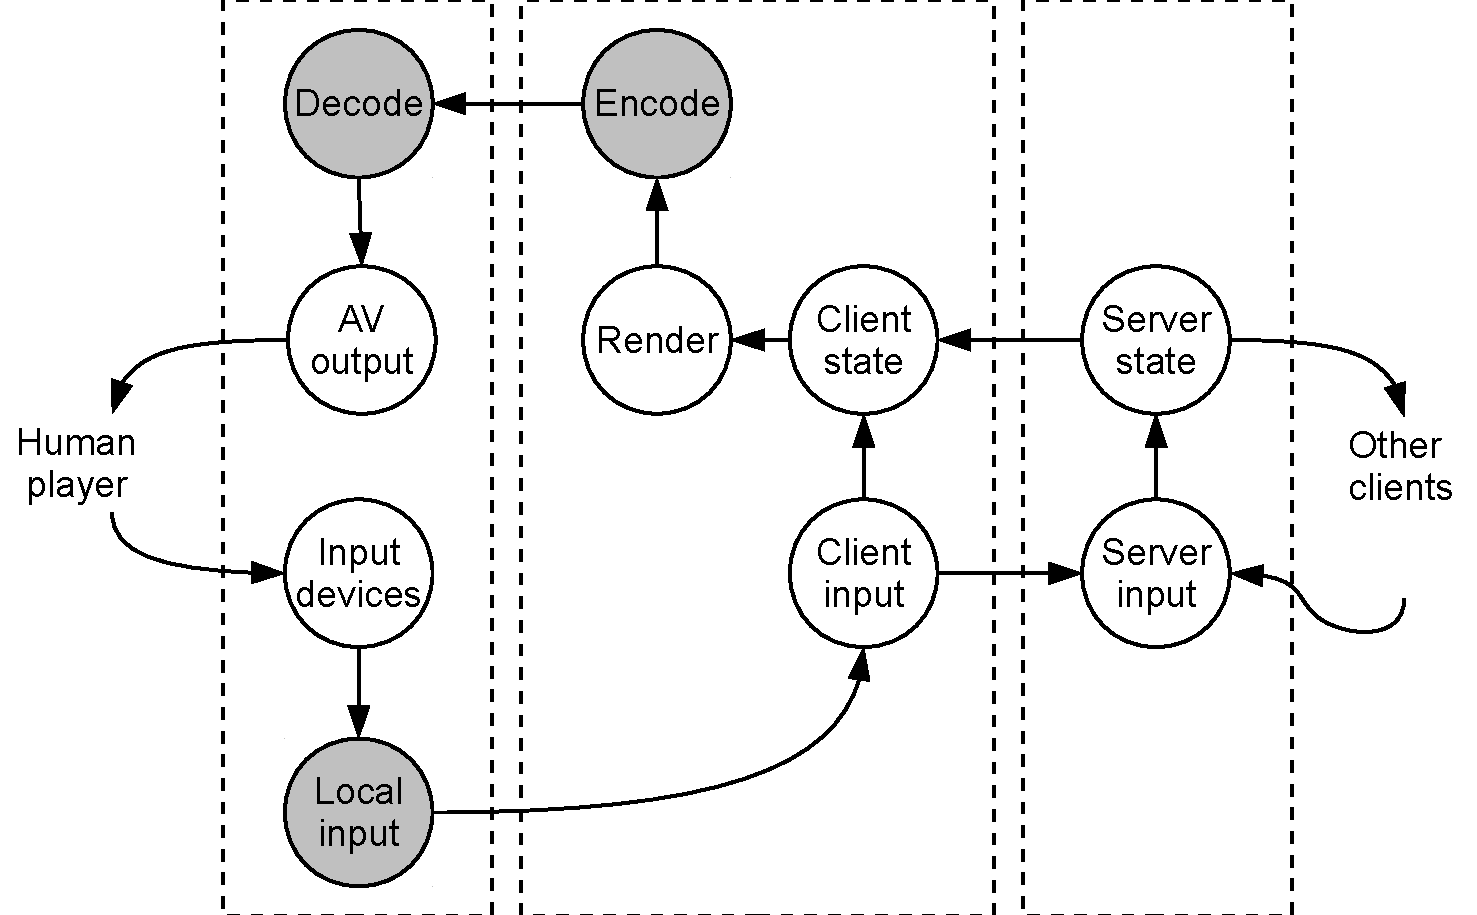
\includegraphics[width=0.8\columnwidth]{../models/component_interaction-online+cloud.pdf}
%   \caption{Interaction of TODO.}
%   \label{fig:component-model-online+cloud}
% \end{figure}

% \begin{figure}
%   \centering
%   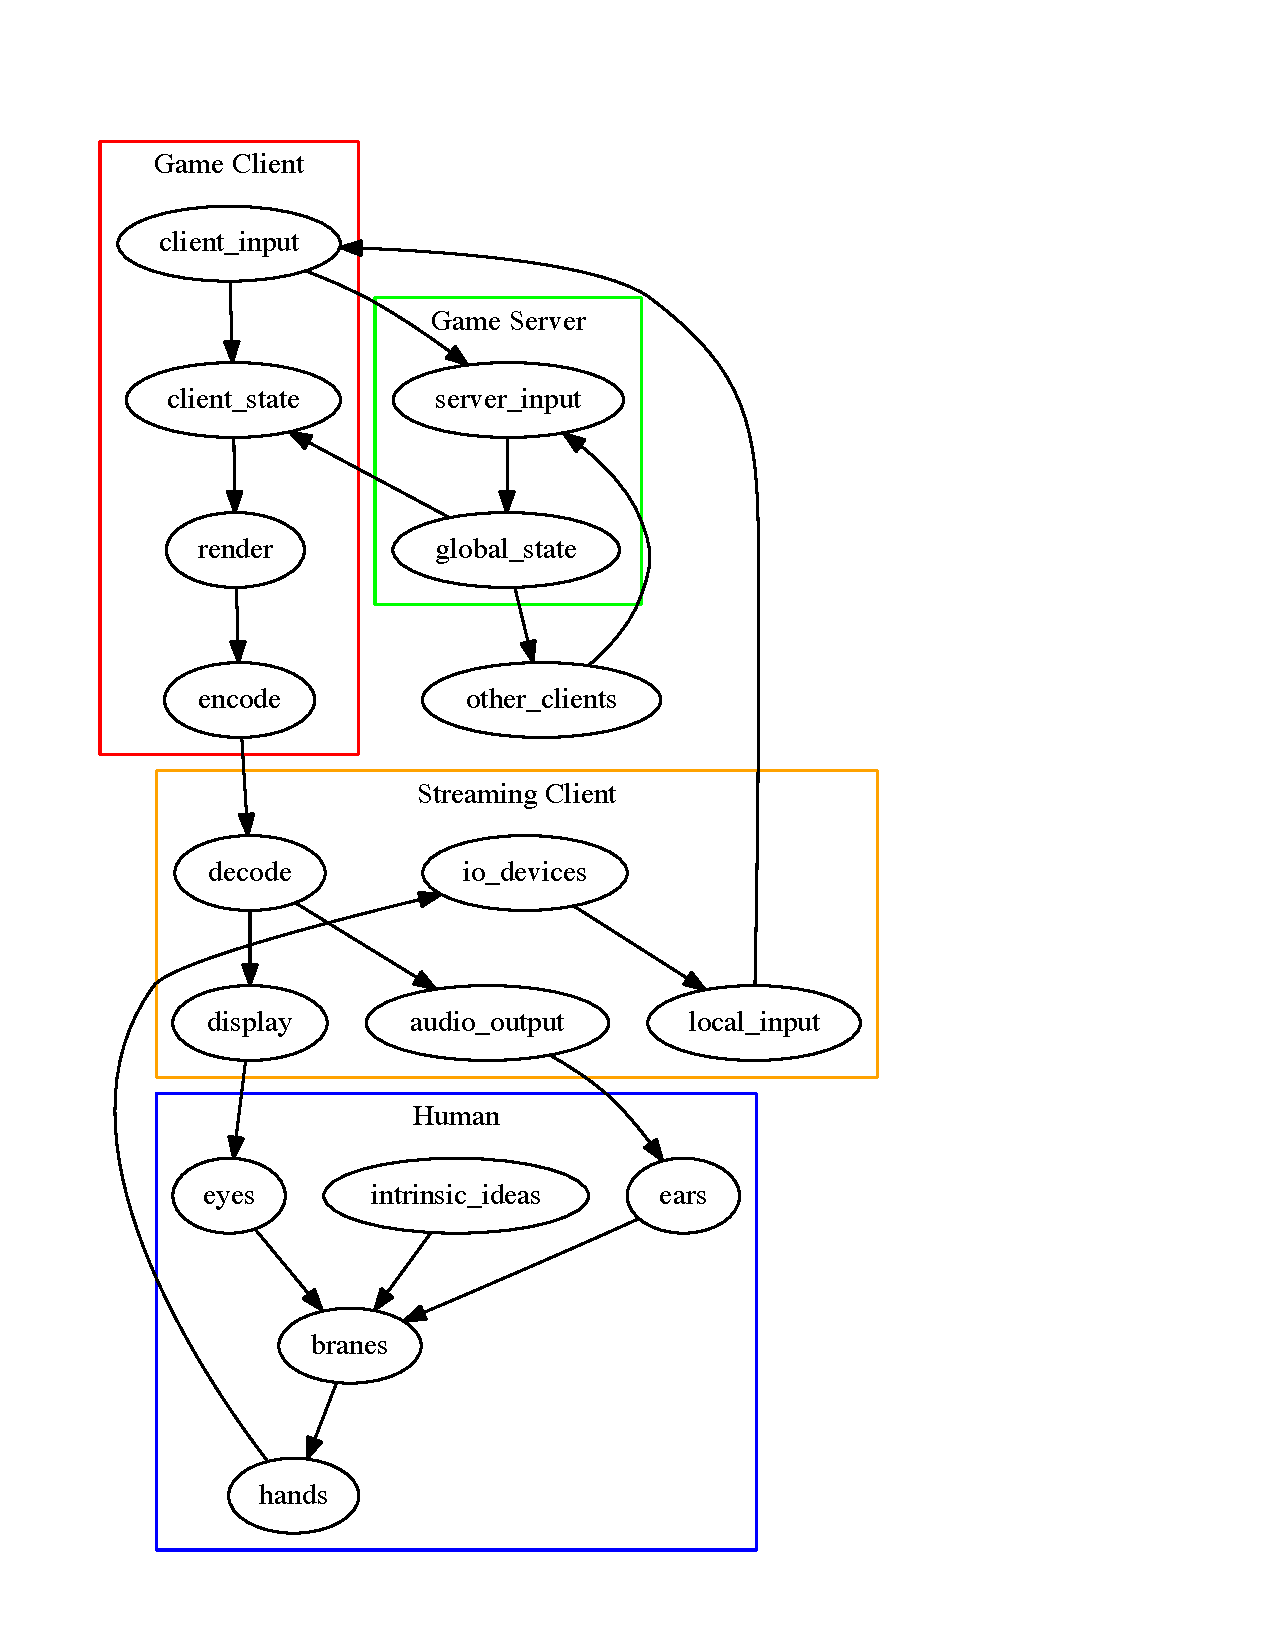
\includegraphics[width=1.0\columnwidth]{../models/cycle.pdf}
%   \caption{Interaction of TODO.}
%   \label{fig:component-model}
% \end{figure}





%Generally speaking, motion in video data is based on the principle of \textit{apparent motion}. In order to perceive objects to be in motion in videos, consecutive images have to appear at a certain rate which is considered to be at about \SI{16.67}{\hertz} according to \cite{wertheimer1912experimentelle}. Below that threshold objects will appear as two distinct objects between two consecutive frames. %This form of apparent movement is called the phi phenomenon. The higher the rate of displaying images, the more fluid the motion looks, as the discrete ``jumps'' in the position of the object get smaller the higher the framerate is.\footnote{One can verify this behavior for example at \url{https://frames-per-second.appspot.com/}.}.

% In general, there is no commonly established upper limit to the framerate that humans can still perceive as an improvement to motion presentation, the gain has however diminishing returns. The typical movie framerate of \SI{24}{\hertz} is considered to be at the lower end of motion perception but mostly still works without any problem due to the presence of motion blur. This artifact is always present in recorded images as objects are still in motion during film exposure. %A faster shutter speed reduces the amount of motion blur. % film grain also has an influence

% \begin{figure}[!t]
% 	\centering
% 	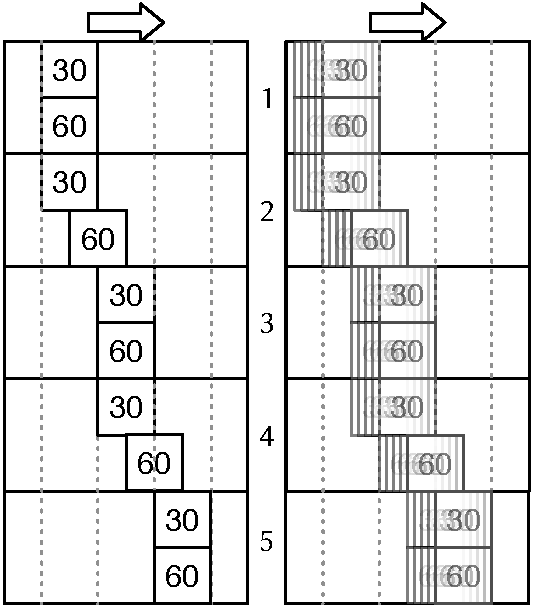
\includegraphics[width=1.0\columnwidth]{images/framerate.pdf}
% 	\caption{Effects of frame rate and motion blur on the smoothness of movement and spatial resolution. Objects move at the same speed to the right only the position os updated at different rates. A depiction of strong motion blur was added to the right-hand side.}
% \label{fig:framerate}
% \end{figure}

% The benefit of motion blur lies in its ability to conceal stutters in apparent movement due to the object and its edges being blurred, thereby reducing the positional information available on it.%, Figure~\ref{fig:framerate} illustrates this. 
% Therefore, typical movie sequences usually appear to be perfectly fluid. Only for example when the camera pans at a high speed stutters in object movement or the viewport updates become apparent. Intrinsic motion blur is absent in computer generated imagery but can be artificially added to the images. While adding blur to video games can improve fluidity, it also reduces the spatial information available to the player and hampers the precision of the player's actions. Therefore it is often avoided, especially for objects in focus.

% Video games add two more factors to the frame rate consideration. The first is the issue of the monitor's refresh rate. Monitors work with a fixed, configurable image refresh rate, typically always including \SI{60}{\hertz}. If the game outputs images at an inconsistent rate or a rate lower than the monitor's refresh rate or if the framerate is not an integer multiple of the refresh rate or vice versa one of two things will happen: tearing or stuttering. % TODO: shorten and rephrase this section

% \begin{itemize}
% 	\item If the monitor fetches a frame from the graphics card's buffer while the frame is still being rendered, the result will be a mixture of the new frame in the upper half of the image and a frame which is one time interval older. This artifact is called \textbf{tearing} and should be avoided.
% 	% only the upper portion of the frame  finished, One frame split up between two refresh cycles
% 	\item Games can also be configured to postpone the rendering of a new frame until the monitor has already fetched and displayed the current frame, this is called waiting for vertical synchronization or \textbf{VSYNC}. No tearing will occur, but the \gls{IAT} of new frames might become very irregular, displaying some frames more often than others just to match the monitors refresh rate, resulting in a stuttering display. This latter stuttering effect also occurs for \SI{24}{\hertz} movies being displayed on a \SI{60}{\hertz} TV screen. Therefore most TVs additionally provide a dedicated \SI{24}{\hertz} refresh rate mode to remove the stuttering.
% \end{itemize}
%!TEX root = paper.tex
%%%%%%%%%%%%%%%%%%%%%%%%%%%%%%%%%%%%%%%%%%%%%%%%%%%%%%%%%%%%%%%%%%%%%%%%%%%%%%%%
\section{Related Work}
\label{sec:relatedwork}


The assessment of video games has been a topic in many past papers. Due to the strong interactivity of games and the large number of different game mechanics most of the research is focused on conducting user studies and noting the subjective quality of the users. But the outcome of these studies still depends very much on a wide selection of factors, e.g., on the precise setup, the game, and the choice of players, that make comparing their results to each other quite difficult. This section presents a few examples of such studies.

In \cite{5976180} Jarschel et al. identify some influence factors on the subjective quality of cloud gaming through a user survey for certain games and three different game categories (slow, medium, fast games) that have been subjected to worsening \gls{QoS} parameters. Downstream packet loss and delay was noted be be especially problematic for achieving a good quality. Similarly, the authors of \cite{4591393} observed the relationship of players quitting a \gls{MMO} game with deteriorating \gls{QoS} and noted an impact proportion of 1:2:4:3 for delay, jitter, and packet loss on both the client-to-server and server-to-client connections respectively. Additionally, a user study in \cite{4604397} also showed a correlation of the \gls{QoE} to the delay as well as the jitter for another \gls{MMO}, in this case the total delay had more impact than the delay variation. Regarding the subjective quality in first person shooters, the authors of \cite{6614351} find a strong impact of the delay and packet loss on the experienced quality. The authors of \cite{6404025} and \cite{beyerusing} use \gls{fEMG} and \gls{EEG} approaches respectively to examine individual gamers' reaction to various cloud games and measure the quality they are experiencing in terms of real-time strictness and \gls{QoE}. Finally, an ITU-T Recommendation \cite{mollertowards} concerning subjectively measuring video game \gls{QoE} is also in preparation, which discusses game-relevant \gls{QoS}-metrics as well as the selection of players and games.

In order to avoid some of the issues with subjective user studies other approaches examine the players' objective performance through in-game metrics such as the game's highscore or the duration to achieve a certain task. For example, a user study in \cite{Chen:2006:SOG:1167838.1167859} observes a decrease in the objective quality assessment metrics (the playing duration) in an \gls{MMO} due to the influence of network factors. A 2006 paper \cite{Claypool:2006:LPA:1167838.1167860} categorizes player actions and their relationship to latency, with special regards for the actions' precision as well as their deadline. However, the in-game metrics under study can not represent short-term effects of latency as they operate on much larger time-scales. 
%(e.g. researching the whole technology tree in Warcraft 3 is neither a representative action of the game nor delay-sensitive at all). Also the presence of lag compensation techniques is not considered. The end result is a delay tolerance table which probably is not very representative of modern video games.
A second paper by Claypool et al. \cite{claypool2007} furthers this notion of the influence of network \gls{QoS} on in-game actions and specifically looks at players' performance in first person games. A user study records the performance in artificially created in-game environments. Here, the performance gets worse with a degraded network, albeit at a very slow pace. %Players were also subjected to very low framerates of \SI{7}{\hertz} and \SI{3}{\hertz}, which is such an unrealistic setting, that it should not even have been tested. The reasons for this are laid out in Section~\ref{sec:framerate}.
The ``kills per minute'' of normal players in the \gls{FPS} \textsc{Quake 3} are investigated by \cite{1266180}, which sees a steady decline of this subjective performance metric when increasing the network delay. However, another paper \cite{Beigbeder:2004:ELL:1016540.1016556}, looking at player performance in \textsc{Unreal Tournament 2003} in a controlled in-game environment, finds almost no influence of increased delay and packet loss, even at high values of \SI{200}{\milli\second}. %The discrepancy between the otherwise similar studies could potentially be attributed to the specific construction of the in-game test environment. 
A 2002 paper \cite{Pantel:2002:IDR:507670.507674}, which gathered objective \gls{QoE} measurements from a custom-made RC racing video game, again sees a strong dependence of the player's performance on the delay, and suggests that a network \acrshort{RTT} of \SI{200}{\milli\second} is barely usable and \SI{500}{\milli\second} completely unusable. Finally, the authors of \cite{Bredel:2010:MSR:1944796.1944797} also find a strong and negative influence of high delay on the player's performance, in this case again in \textsc{Quake 3}. 

It is interesting to note the discrepancies both in terms of the influencing parameters as well as their degree in between the studies. Considering the complexity and variability of video games and the difficulties of finding and setting up good comparable scenarios and testbeds, it is understandable that some studies come to different results. This makes it much more important to first understand the basic components and underlying objective metrics. Quality estimations of video games could be much more representative if models for these metrics would exist to easily understand their influences without having to conduct a full user study.





%Pure \gls{QoS} views on the quality of online video games are rather are, but are nonetheless important in correctly assessing any game-related parameters and are also the foundation for most objective and subjective \gls{QoE} studies.



%A 2012 article notes the dependence of gaming on latency and the difficulties cloud-based solutions have in providing a sufficiently low latency. The suggest a move closer to the edge to reach more users in a quality they deem adequate.  \cite{Choy:2012:BSC:2501560.2501563}.
%``The Brewing Storm in Cloud Gaming: A Measurement Study on Cloud to End-user Latency'' 

%``Placing Virtual Machines to Optimize Cloud Gaming Experience'' \cite{6853364}  interesting for cloud gaming economics

%Adaptive Mobile Cloud Computing to Enable Rich Mobile Multimedia Applications \cite{6413270}

%Addressing Response Time and Video Quality in Remote Server Based Internet Mobile Gaming \cite{5506572} optimize mobile cloud gaming based on a certain impairment function and by reducing video bitrate and fps (even sub 10fps...)

%``Kahawai: High-Quality Mobile Gaming Using GPU Offload'' \cite{Cuervo:2015:KHM:2742647.2742657}

%``Outatime: Using Speculation to Enable Low-Latency Continuous Interaction for Mobile Cloud Gaming'' \cite{Lee:2015:OUS:2742647.2742656}

%``Assessing the Impact of Game Type, Display Size and Network Delay on Mobile Gaming QoE'' \cite{beyer2014typedisplaydelayimpact} Another user study regarding context factors like screen size and their impact on MOS, but also game type and delay on MOS

%A Method For Feedback Delay Measurement Using a Low-cost Arduino Microcontroller \cite{beyermethod} already covered in measurement methods section

%``QoE Assessment of Interactivity and Fairness in First Person Shooting with Group Synchronization Control'' \cite{Ida:2010:QAI:1944796.1944806} interessant für lag compensation betrachtungen

%``The Impact of Video Encoding Parameters and Game Type on QoE for Cloud Gaming: a Case Study using the Steam Platform'' \cite{slivarimpact}

%``How Do New Visual Immersive Systems Influence Gaming QoE?'' \cite{hupontnew} Vergleich Immersion am monitor vs oculus. beispiel eines schlechten testsetups, da unterschiedliche FoV für beide ausgabetypen (75° vs 100°), test wird stark verfälscht

%%``An experimental estimation of latency sensitivity in multiplayer Quake 3''  vs. \cite{1266180} ``The Effects of Loss and Latency on User Performance in Unreal Tournament 2003'' \cite{Beigbeder:2004:ELL:1016540.1016556}. both papers completely contradict each other: Quake 3: significant impact of latency on game performance (kills/minute); UT3: no impact on user performance at all (kills/deaths per game)

%``Security issues in online games'' \cite{doi:10.1108/02640470210424455}
%!TEX root = paper.tex
%%%%%%%%%%%%%%%%%%%%%%%%%%%%%%%%%%%%%%%%%%%%%%%%%%%%%%%%%%%%%%%%%%%%%%%%%%%%%%%%
\section{An End-to-End Lag Model}
\label{sec:model}

It is evident from the discussion in Section \ref{sec:background} 
that multiple different components contribute to 
the end-to-end lag in games, and that multiple potential models and 
levels of granularity exist for each game type.
Let's discuss therefore the model boundaries and level of detail 
used in the current iteration of this analytical model to be presented here.

First, we define the end-to-end lag to be the time elapsed 
from when the player supplies commands to the input devices until just 
before actual audio/video output.
% I.e.: rendering, *and* encode/decode for cloud games
We assume that the actual presentation of 
audio and video content happens instantaneously  
(ignoring any screen synchronization issues), and assume the player 
input to be a stochastic process. % future work!1!!
Furthermore, as also found in practice, input events are queued up  
and sent en bloc at a specific, configurable interval.

Second, in our treatment of client-server games, we focus on modeling 
a single connected client and its interaction with the game server. 
While other clients might be connected to the same server, it is 
solely the server that controls when game state updates are sent. 
Thus, the client we are looking at does not need to account for the 
behavior of other clients.
% probaby not future work

Next, we associate a static (but individually parametrizable) tick 
rate with the computation process of the game server, and a frame rate 
with the render process. 
The server updates the state of the game world at every tick, and may 
spend some processing time in order to do so. Once finished, an update 
message is sent to the client.
Independent of the update process, the game client outputs the next 
video frame in accordance to the frame rate. The game client's state 
might not get updated by the server between rendered frames. Still, 
output is generated\footnote{A practical game implementation will use state prediction for this.}.

Note that while the delay between frames is held constant here,
the lag between an input event and the earliest frame containing a perceptible 
result of that event can take multiple frame times.

While we consider the command, tick, and frame rates to be constant 
(while not necessarily identical), there is no inherent synchronization 
between them. This is represented in the simulation by a random initial 
phase offset for each of the rates.

Finally, since we are simulating online games, the simulation obviously 
includes the network paths between the different components. The delay 
distributions are freely configurable, but may be omitted entirely as well.
Fig.~\ref{fig:queuing-model} gives a graphical representation of the model for the online video game case.

\begin{figure*}[!t]
	\centering
	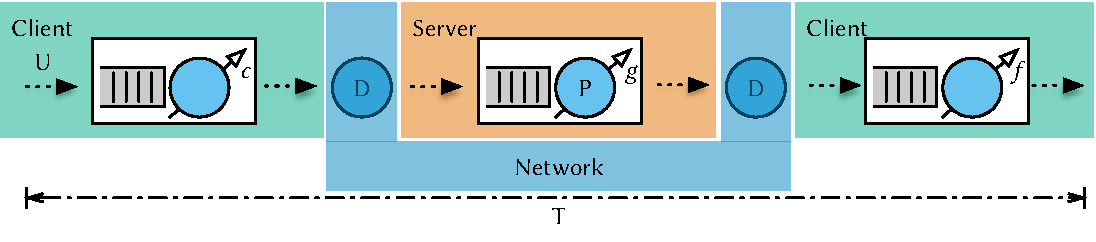
\includegraphics[width=1.0\textwidth]{../models/e2e-lag-model.pdf}
	\caption{Abstract end-to-end lag queuing model representation in the online video game case.}
\label{fig:queuing-model}
\end{figure*}



\subsection{Model simplifications}

The simulation model at hand does not attempt to capture all possible 
sources of lag that. Indeed, we simplify the model in the 
following aspects in the hope to make the results more tractable.
%\textbf{TODO Make this more of a ``future work'' section, less ``why we suck''.}

\paragraph{Additional delay sources.}
The simulation ignores, i.e. 
models as a constant zero contribution, the delays contributed by 
input devices like keyboards, mice, and game controllers. We estimate 
these at below \SI{10}{\milli\second}. The same goes for the  lag of 
the display device (from after rendering or decoding until the frame 
is actually visible) which is typically in the range of 1--3 frames for a computer 
monitor, and larger for TV sets. 
% TODO: \textbf{Add adaptive VSYNC?}

\paragraph{Subtleties of game internals.}
Modern games go great lengths 
to handle lag gracefully, and try to ``work around it'' in various ways. 
The methods for this vary, and implementations usually are not open 
for examination, so we leave them for further study. 
Techniques include lag compensation (the game client 
tries to predict the server state from past knowledge, allowing for 
smoother local updates but possibly causing slight deviation and 
re-synchronization artifacts), and tick- and framerate adaptation 
at the game server and client, respectively.
Lastly, player actions in a game might take multiple command time 
intervals to perform. The simulation currently assumes that every 
single batch of commands that reaches the server will result in 
state updates and thus changes in the perceptible output of the game 
client. It should be noted, that none of these techniques alter the 
end-to-end lag itself, rather they just try to conceal it on some higher level. 
Therefore, the mechanisms do not invalidate our examination of the basic 
end-to-end lag itself.
%\textbf{TODO I'm making this up. PLX correct.}

\paragraph{Factors in human perception and strategy.}
The lag model 
we present does not take into account the perceived lag from when the 
player \textit{thinks} they have triggered an action to when they 
perceive the outcomes of their action. This consequently disregards 
effects of different player actions (``traverse vs fight''), strategies 
(``assault vs snipe''), and so on.





%%%%%%%%%%%%%%%%%%%%%%%%%%%%%%%%%%%%%%%%%%%%%%%%%%%%%%%%%%%%%%%%%%%%%%%%%%%%%%%%
\subsection{Sources of Latency in Gaming}
\label{sec:latency}


Fig.~\ref{fig:tickrate-timeseries} shows a time series attempting to exemplify this for the simplified case of an online video game.

\begin{figure}[!t]
	\centering
	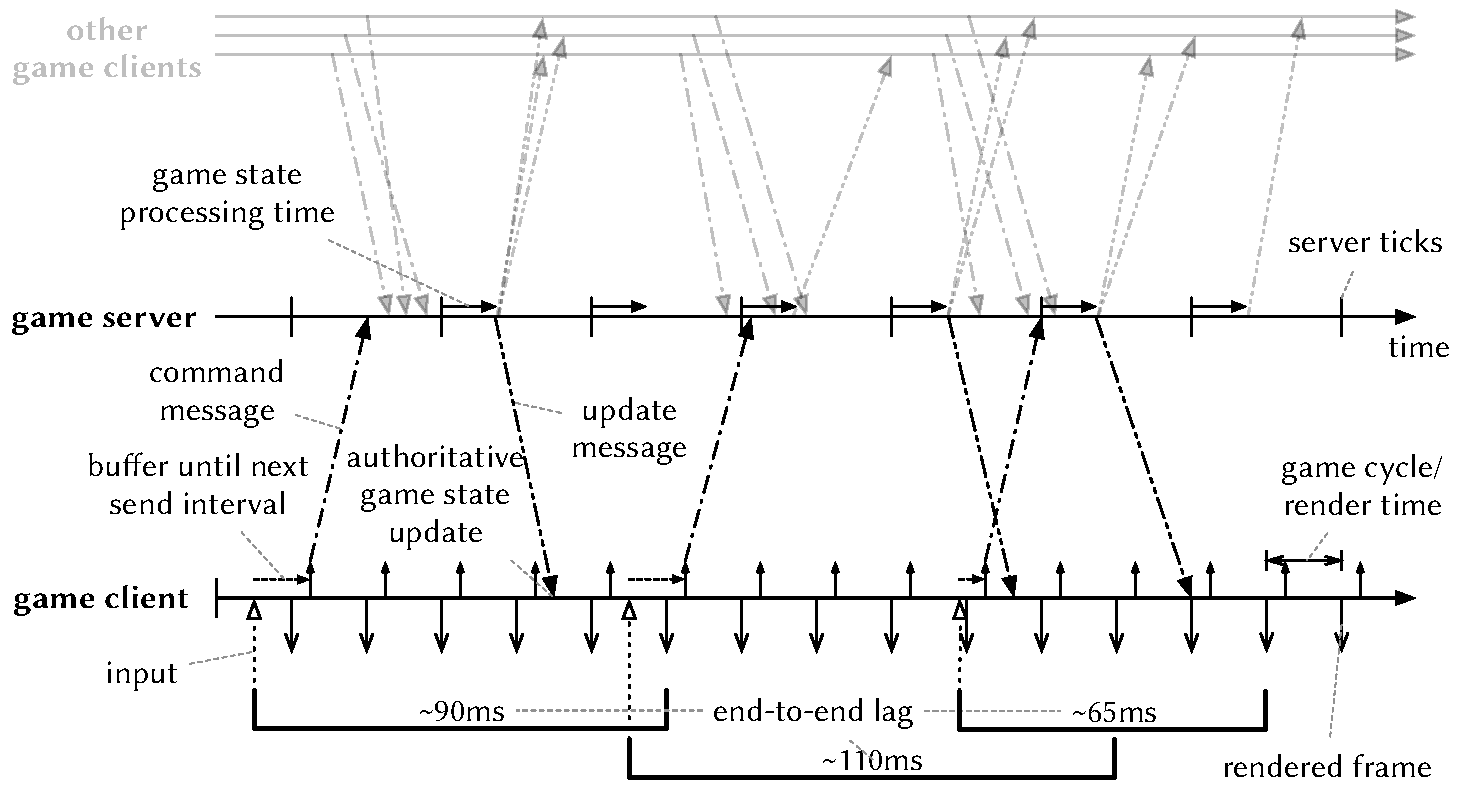
\includegraphics[width=1.0\columnwidth]{../models/tickrate-timeseries.pdf}
	\caption{Exemplary flow of events in online client-server game, and resulting end-to-end lag. Delay values are given for a framerate of \SI{60}{\hertz} and a server tickrate of \SI{30}{\hertz}, the network latency will only show minor variations.}
\label{fig:tickrate-timeseries}
\end{figure}



%All in all, if possible, video game measurements should always consider the full \textbf{end-to-end} lag factoring in every possible source of delay but also the presence latency compensation and concealment techniques.



% Online games attempt to compensate network latency through various means, such as already showing the results of your local inputs while waiting for the authoritative update from the server and potentially rolling back the local updates.

% TODO: Also mention lag compensation/concealment techniques:
% Client-side: non-authoritatively update game state based on own inputs and merging it afterwards with the server's view, correcting any prediction errors
% Server-side: Keep a short history of past game states, and do not execute player commands at the state they were received but rather at the (estimated) state time they were intended for.

% lag compensation can also be implemtented specifically for cloud gaming as the work conducted in \cite{Lee:2015:OUS:2742647.2742656} suggests, however incurring siginficant overhead in terms of processing time for the game logic and renderer as well as the encoding and bandwidth due to specutatively generating and transmitting frames ahead of their corresponding input.


% game keeps history of recent game state snapshots to interpolate between two server states and create a smoother experience (thus decoupling client frame rate from the server's state updates), but adds e.g. \SI{100}{\milli\second} of view lag due to snapshot history.


%%
%\subsubsection{Online Video Game Latency Concealment Techniques}


% input: absolute (eg mouse) vs. relative (analog stick)
% frame perfect input
% double/triple buffering
% inputs per minute vs timing precision of input
% range of interactivity
% latency sensitivity/responsiveness of different game mechanics / UI elements in the same game
% latency of camera movement / UI vs actual game elements


%Info on source engine networking: \url{https://developer.valvesoftware.com/wiki/Source_Multiplayer_Networking}
%\url{https://developer.valvesoftware.com/wiki/Latency_Compensating_Methods_in_Client/Server_In-game_Protocol_Design_and_Optimization}
%(Latency Compensating Methods in Client/Server In-game Protocol Design and Optimization, Yahn W. Bernier (yahn@valvesoftware.com), 2001, Software Development Engineer, Valve Software)



% Online games generally follow one of two designs. Either there is a dedicated server available to host the game, or one of the clients is elected to additionally act as the server.
% The election is typically based on criteria such as the available performance and latency. If the selected host drops out of the game, a new server has to be elected and the game gets migrated there, usually stopping the game for a few moments. Competitive games almost always choose the dedicated approach to ensure fairness, stability and better control cheats.



% \begin{figure*}[!t]
% 	\centering
% 	\begin{subfigure}[b]{0.5\textwidth}
% 		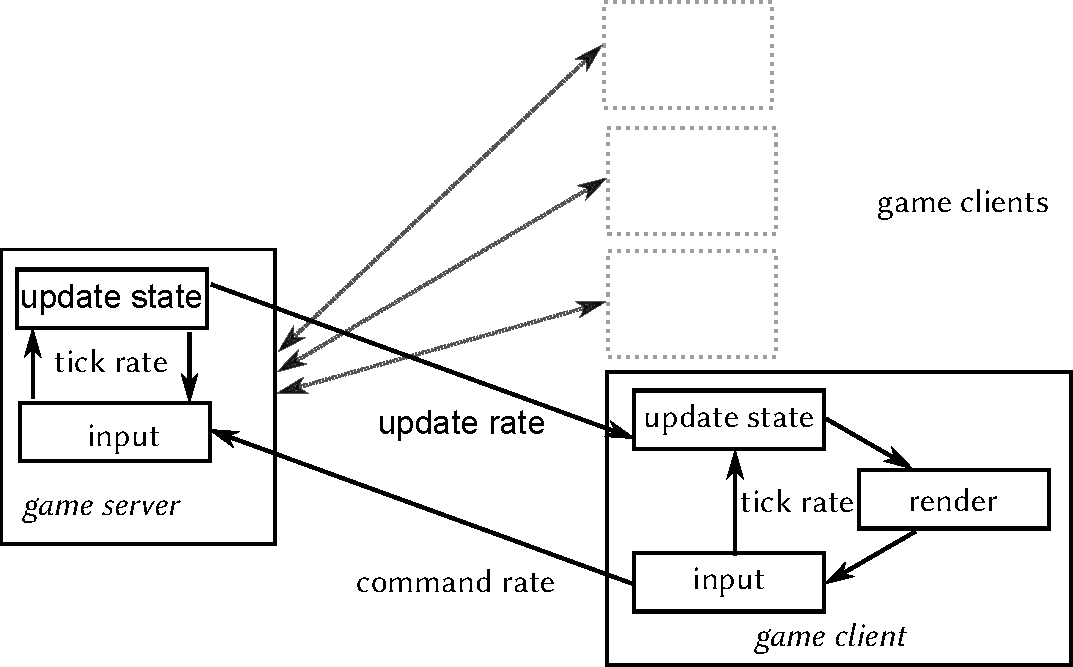
\includegraphics[width=1.0\columnwidth]{images/game-tick-rate.pdf}
% 		\caption{In typical online games.}
% 		\label{fig:tickrate-online}
% 	\end{subfigure}%
% 	~
% 	\begin{subfigure}[b]{0.5\textwidth}
% 		\includegraphics[width=1.0\columnwidth]{images/game-tick-rate-streamed.pdf}
% 		\caption{In a cloud gaming scenario.}
% 		\label{fig:tickrate-streamed}
% 	\end{subfigure}
% 	\caption{Interaction of the game client and server.}
% 	\label{fig:tickrates}
% \end{figure*}



% \begin{figure}[!t]
% 	\centering
% 	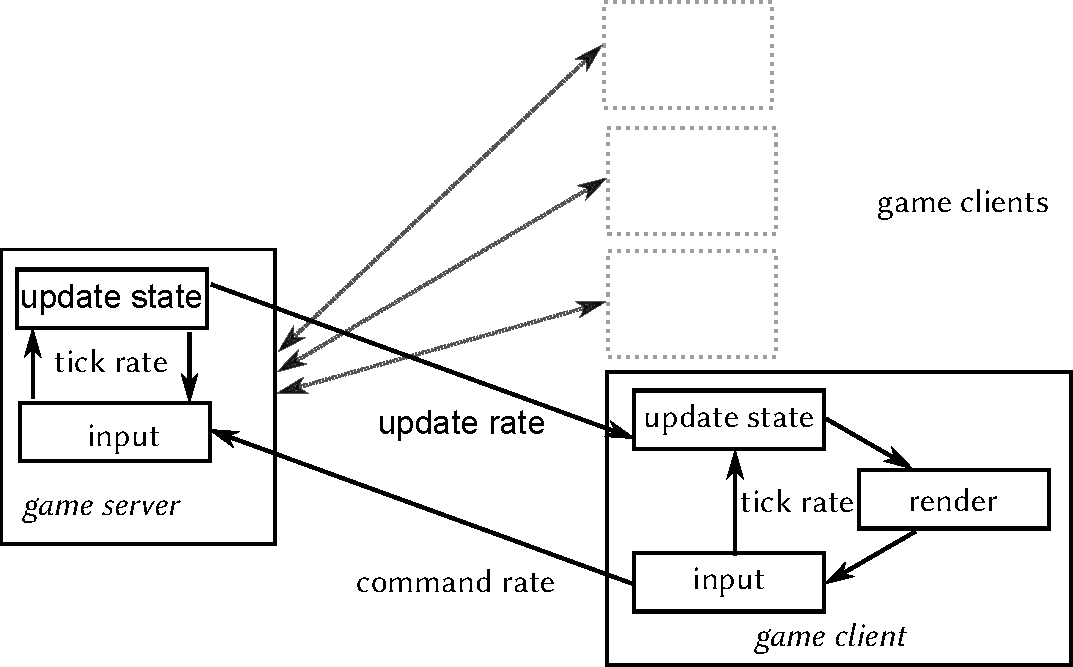
\includegraphics[width=1.0\columnwidth]{images/game-tick-rate.pdf}
% 	\caption{Interaction of client and server in typical online games.}
% \label{fig:tickrate-online}
% \end{figure}








% \subsection{Determining Video Game Popularity and Engagement}
% FUTURE WORK!

% Using Steam data as a popularity measure and get a grasp of which games could be worthwhile to look at. Ties in to user engagement metrics to determine the quality a game delivers in a current situation. Alternative view: the more engaged players are to a game, the more important is delivering a good quality (e.g. for streaming).

% For example, there might be a correlation between a game's price and the average time it's been played, as Figure~\ref{fig:tickrate-streamed}.


% Other  k-means clustering of steam/price data or other graphs

% \begin{figure}[!t]
% 	\centering
% 	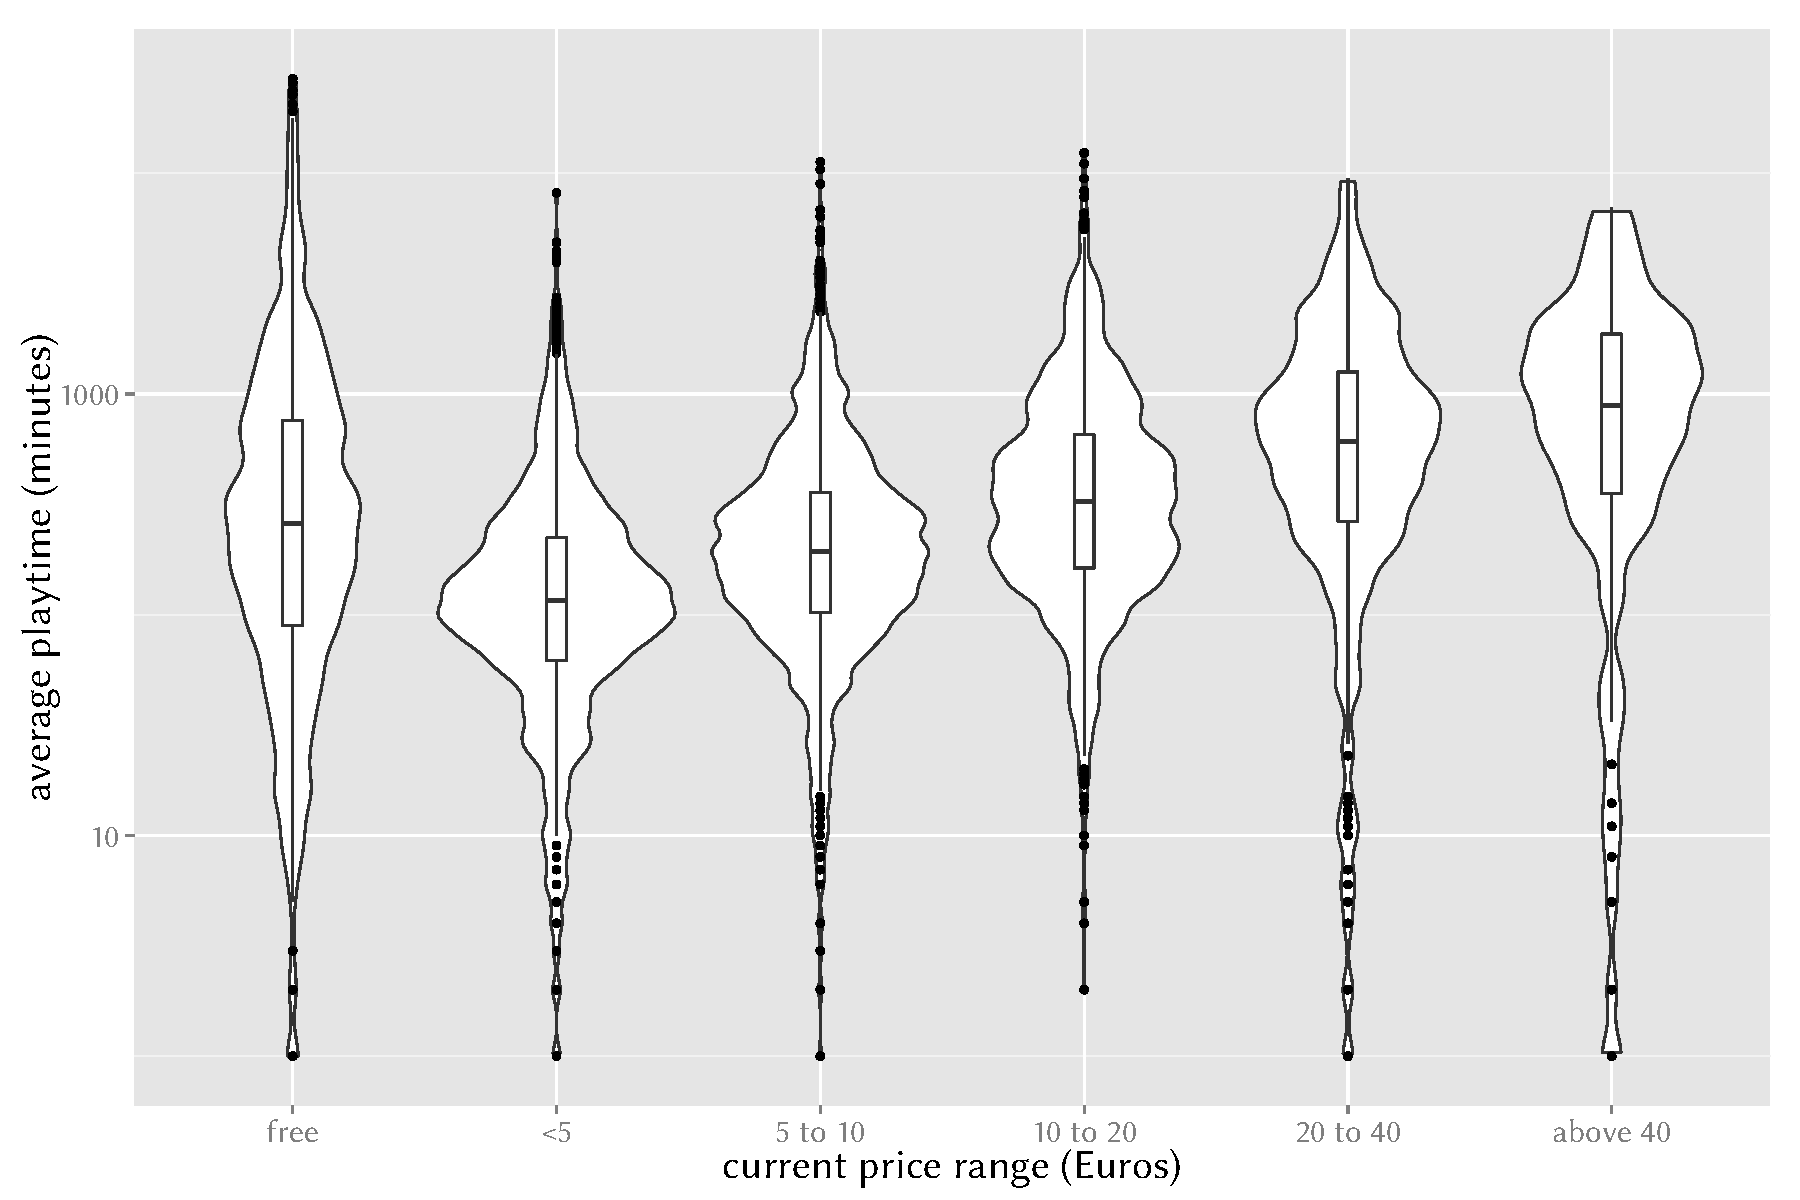
\includegraphics[width=1.0\columnwidth]{images/dampfviolinen-playtime.pdf}
% 	\caption{Game cost as a possible categorization and engagement factor. Displayed is a violin plot of the current costs in relation to the average playtime of individual games.s}
% \label{fig:cost-playtime-violin}
% \end{figure}

% Categorization dimensions viable for measuring online video game quality:



%\footnote{\url{http://accidentalscientist.com/2014/12/why-movies-look-weird-at-48fps-and-games-are-better-at-60fps-and-the-uncanny-valley.html}}
%\url{https://stackoverflow.com/questions/17411/how-do-you-separate-game-logic-from-display}
%\url{http://higherorderfun.com/blog/2010/08/17/understanding-the-game-main-loop/}

%!TEX root = paper.tex
%%%%%%%%%%%%%%%%%%%%%%%%%%%%%%%%%%%%%%%%%%%%%%%%%%%%%%%%%%%%%%%%%%%%%%%%%%%%%%%%
\section{Simulation and Scenario Evaluation}
\label{sec:simulation}

Based on the models introduced in Section~\ref{sec:model} a stochastic \gls{DES} was created. This \textsc{Gnu R}-based simulator strives to translate all of the earlier discussed components of lag, while keeping them as configurable as possible.
%By using a vector-based language the core loop is kept compact and easy to modify in order to adapt to new scenarios in addition to the ones evaluated here. 
Due to the influence of several stochastic processes (user inputs $U$, network delay $D$, server processing time $P$) and the differing offset of the clocked processes, a sufficient number of repetitions is required to provide meaningful results. This is achieved by running large numbers of simulations in parallel through the built-in R facilities.

This section presents simulation results on each of the flavors of how to play video games: the local, online, and the cloud scenario. The investigations here are not intended to cover every aspect of all parameters or to conduct full parameter studies, but are rather to highlight some particular aspect in each of the scenario.

All of the source code and the data from the upcoming scenarios is provided in the simulation folder\footnote{\url{https://github.com/mas-ude/onlinegame-lag-sim/tree/master/simulation}} of the repository and can be used as public domain.


\subsection{Parameters}

Besides being fully reconfigurable, the simulation currently also has a few default parameters set and makes assumptions that go beyond what the base end-to-end model implies for reasons of simplicity. They are chosen to be as realistic as possible and and are summarized in Table~\ref{tab:notation}.
%\hoss{Vielleicht noch kurz erwaehnen, dass die Parameter realistisch gewaehlt sind? Gibt es dafuer Referenzen?}
% fm: referenzen für solche werte sind leider eher schwer zu finden

First, the input is modeled by an exponential distribution with a rate of $20$ events per second. The offsets between the clocked processes are uniformly distributed in their respective intervals. It is further assumed that the server processing time $P$ follows a left-truncated normal distribution with $\mu_P = \SI{3}{\milli\second}$ and $\sigma_P = \SI{0.1}{\milli\second}$.
%\textbf{TODO:} implications and reasons?
Additionally, the rate $c$ at which command messages are sent to the game server is set equal to the server's tickrate $g$ as the server would not process more commands either way. This might however increase the end-to-end lag in some situations if a command message just misses one of the server's ticks and has to wait another full cycle.

The evaluation of the presented scenarios was conducted on the basis of $r=\np{1000}$ repetitions for each setting. Each run $i \in \{1,\dots,r\}$ consisted of a series of $n=\np{100}$ input events and their associated end-to-end lag $T_{i,j}$ for the $j$-th input event. On this basis a median lag $\widetilde{T_i}$ was calculated over the $n$ input events for each run $i$, and finally an overall mean lag out of the individiual medians of each repetition, i.e. $\overline{T}=\frac{1}{n}\sum_{i=1}^r\widetilde{T_i}$.


%%%%%%%%%%%%%%%%%%%%%%%%%%%%%%%%%%%%%%%%%%%%%%%%%%%%%%%%%%%%%%%%%%%%%%%%%%%%%%%%
\subsection{Local Games}

The first and simplest scenario to be investigated here is the case of the local game. In the version implemented here, the tickrate is still present, but the influence of the network is entirely removed. It therefore represents the best case an online multiplayer game could achieve if the server ran locally. Figure~\ref{fig:nwless-scatter} plots the relationship between the frame duration (i.e., the inverse of the framerate), the tick duration, and the resulting median end-to-end lag.
% NOTA BENE: Every status update that the server sends must wait for another frame time until we consider it rendered.
%
% The scatter plot of raw e2e lag values for one (FR, TR) configuration thus spans
% * separate "boxes" for each CR/FR/TR offset config
% * inside of which the input events U scatter
% * Boxes are, when all other rates/processes are in optimal sync,
%   - bound from below by the frame-time f^-1 as the minimum
%   - bound from above by f^-1 + c^-1, because c "groups together" input events
% * alternatively, when maximally *out of* sync,
%   - the boundaries shift upwards by another f^-1 + g^-1, resulting in a total just short of c^-1 + g^-1 + 2*f^-1: Input event waits almost-full command cycle, which then waits almost-full tick, which then waits almost-full frame; plus one frame per the "nota bene" above.
% * a "cloud of boxes" (per the above description) whose minima are uniformly distributed (from visual inspection).
%
% The distributions of values for different (FR, TR) configs differ in their characteristics pretty starkly:
% * for low framerates and high tickrates, we get an approximately uniform lag distribution. Seems that the FR which is "further down the tandem queue" dominates the lag, so its uniformly distributed phase offset governs the lag distribution.
% * for high framerates and low tickrates, it approaches a truncated normal distribution.
The values can be estimated as follows. Every user input event traverses three queues with fixed-rate outputs ($c=g$, g, and $f$), and every game state update waits for the next full frame until it gets displayed. In the ideal case, an input event occurs just before the command message is sent off, the server tick follows as soon as the message is received, and the update reaches the client just before a frame is output. Then the end-to-end lag is slightly above the frame time that must elapse before the update can be rendered to screen, $T_{min}>f^{-1}$.

In case the events are unfavorably offset against one another, an input event has to wait almost a full command-message cycle until it is sent on; it reaches the server just after a tick has occurred, so it waits almost a full server tick; finally, it will wait for almost two frame times until it is displayed. Combining with the previous result bounds the lag as follows, $f^{-1} < T < c^{-1}+g^{-1}+2f^{-1}$. The mid-interval point between these two limits is $T_{mid}=\frac{3}{2} f^{-1} + g^{-1}|_{c=g}$ which coincides roughly with the medians of the stochastic simulation.


Looking at a typical \SI{60}{\hertz} video game with an equal tickrate (i.e. a frame duration of $\approx \SI{16.6}{\milli\second}$) the median lag is in the range of \SIrange{45}{50}{\milli\second}. So even under quasi-optimal circumstances, there is already a considerable amount of end-to-end lag (even without factoring in the delay of the screen and input devices) that can only increase with the presence of network delay. Therefore, video games (and quality assessments thereof) should try to achieve the highest framerate possible to minimize this influence.

%%%%%%%%%%%%%%%%%%%%%%%%%%%%%%%%%%%%%%%%%%%%%%%%%%%%%%%%%%%%%%%%%%%%%%%%%%%%%%%%
\subsection{Online Gaming}

Next up is the full scenario of an online video game, now with network lag $D$ and server processing time $P$ included. For this exemplary scenario, the one-way delay $D$ was assumed to follow a left-truncated normal distribution, with $\mu_D = \SI{20}{\milli\second}$ and $\sigma_D = \SI{5}{\milli\second}$, producing non-negative network delays. Typical competitive online games today are expected to operate in such ranges. An \acrshort{RTT} of \SI{100}{\milli\second} is often considered to be the upper limit for a good playing experience. $P$ is similarly left-truncated. In addition to the components in the previous scenario, the lag now also contains contributions by the network round-trip and processing delay, $2D + P$.

\begin{figure}[!t]
	% TODO: adjust the bounding box of the 3dbar plot, instead of playing with fire (aka \vspace)
	\centering
	\vspace{-6mm}
	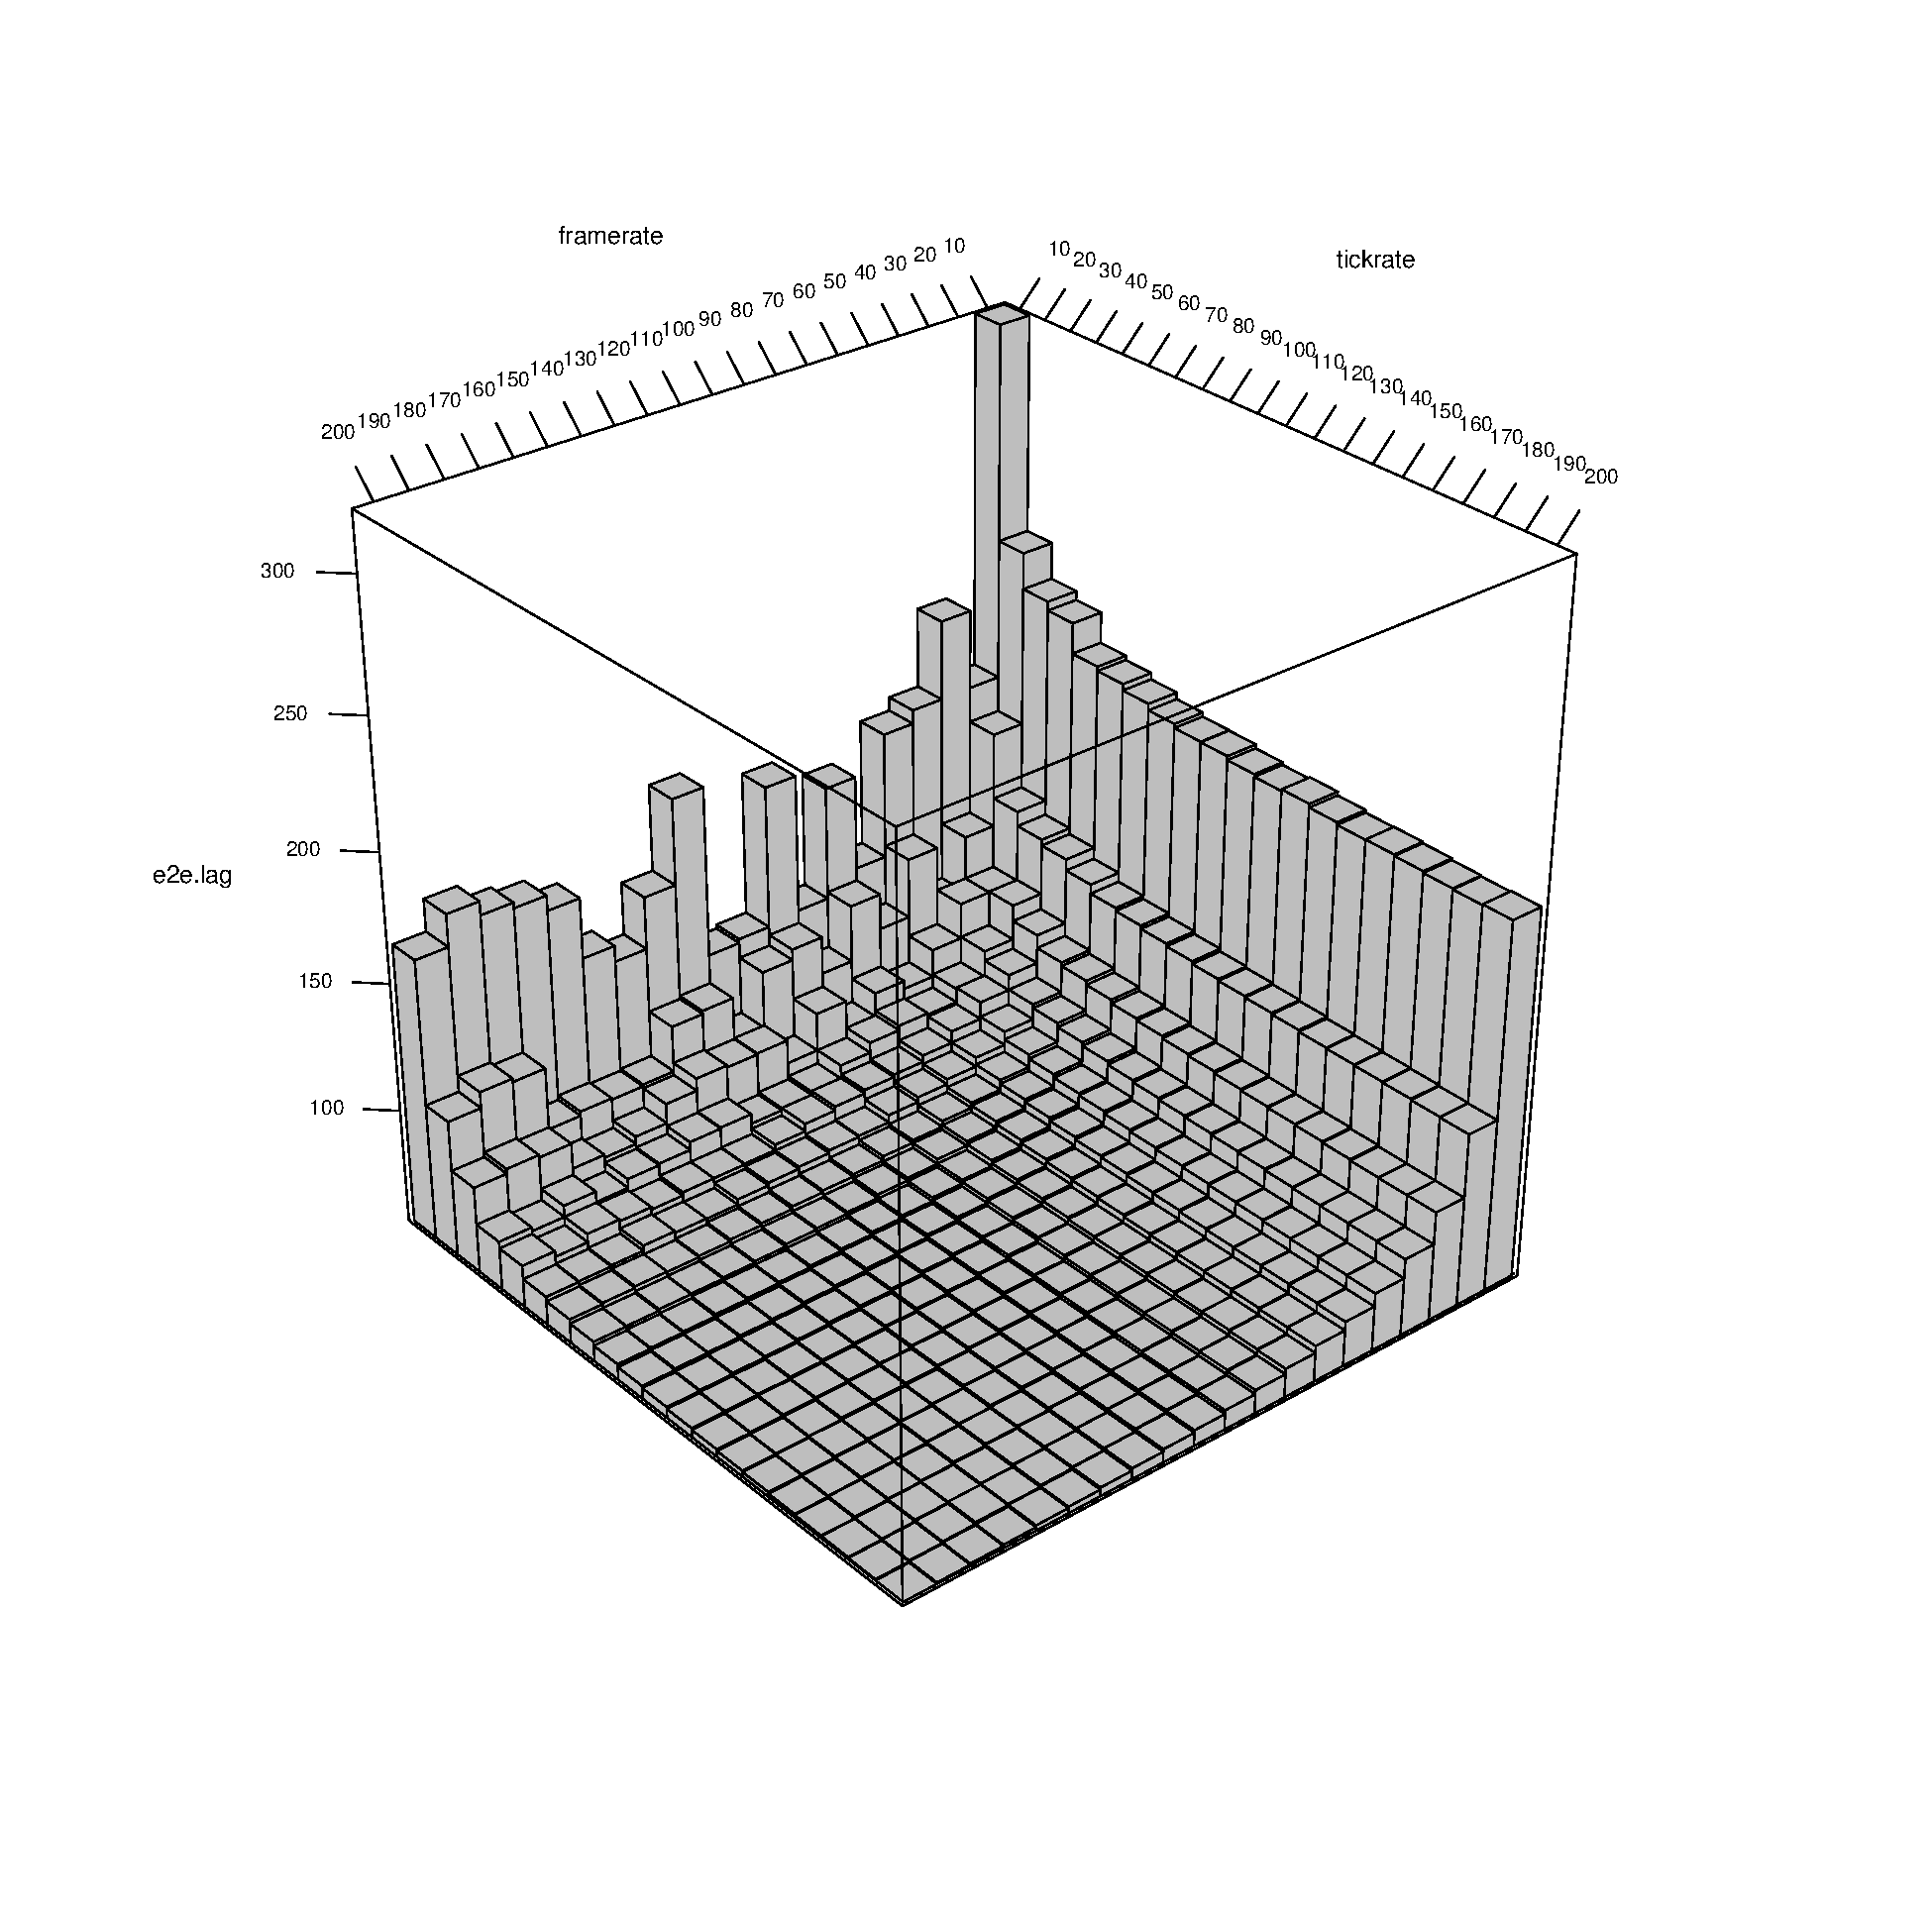
\includegraphics[width=1.0\columnwidth]{../../simulation/visualization/e2e-lag-3dbars.pdf}
	\vspace{-15mm}
	\caption{Influence of client framerate and server tickrate on the median end-to-end lag in the online game scenario. For high rates $f$, $g$, the lag approaches \SI{43}{\milli\second}.}
	% TODO: \hoss{Kann man hier einen stacked bar plot bauen, bei dem man den Networking Anteil sieht? Das wuerde die Aussage gut unterstuetzen.}
	% TODO: nicht rechtzeitig für submission deadline, aber für eine nächste version
\label{fig:3dbars-framerate-tickrate-lag}
\end{figure}

Figure~\ref{fig:3dbars-framerate-tickrate-lag} shows a 3D bar plot of the influence of both the framerate and the tickrate on this scenario. The axes mark typical values for $f$ and $g$. Two things can be noted here. First, the framerate has a larger influence on the lag than the tickrate. Second, for low framerates and tickrates, the impact of network delay on the end-to-end lag is almost completely masked. Only if both rates are high enough, the network delay will play a more significant role. This masking effect has large implications for video games and their evaluation. Many evaluations examine the influence of the network delay only, without considering other contributions to end-to-end lag. Our results indicate that this might not be the best course of action. The effect likely shifts to lower values of the frame- and tickrates when a higher network delay is examined.

Another interesting result (not plotted here) is the much larger variance of lag in the framerate dimension when compared to the tickrate. This requires video game studies to have a very high repetition rate to provide meaningful results.


%%%%%%%%%%%%%%%%%%%%%%%%%%%%%%%%%%%%%%%%%%%%%%%%%%%%%%%%%%%%%%%%%%%%%%%%%%%%%%%%
\subsection{Cloud Gaming}

Finally, we construct a Cloud Gaming scenario. The tickrate has been removed;  instead, a constant encode ($e$) and decode ($d$) delay is in place at the game streaming server and client respectively. The frames are now rendered by the server, so they need to be transported back to the client first. Instead of assuming a specific network throughput and frame size, we simply add one frame time to account for the transmission of the encoded screen contents.
%Without knowing the connection's throughput and absolute values for the frame sizes, the simulation simply applies an upper limit for the transmission duration, namely once again the frame's duration, or the inverse of the framerate. 
For the network delay $D$, the same values as for the online game are used. $c$ is set to $\SI{200}{\hertz}$.

\begin{figure}[!t]
	\centering
	%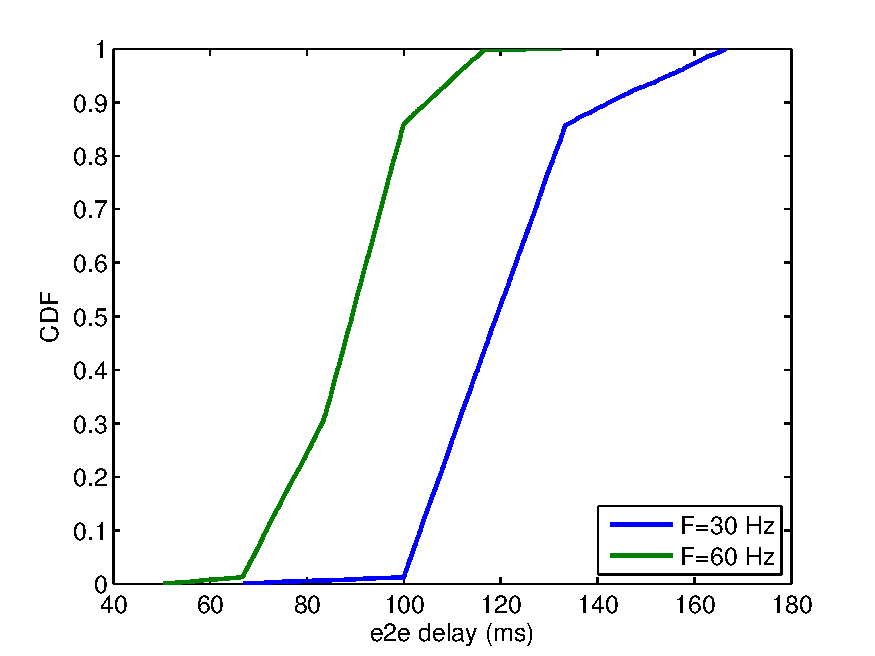
\includegraphics[width=1.0\columnwidth]{images/e2e-delay-sim.pdf}
	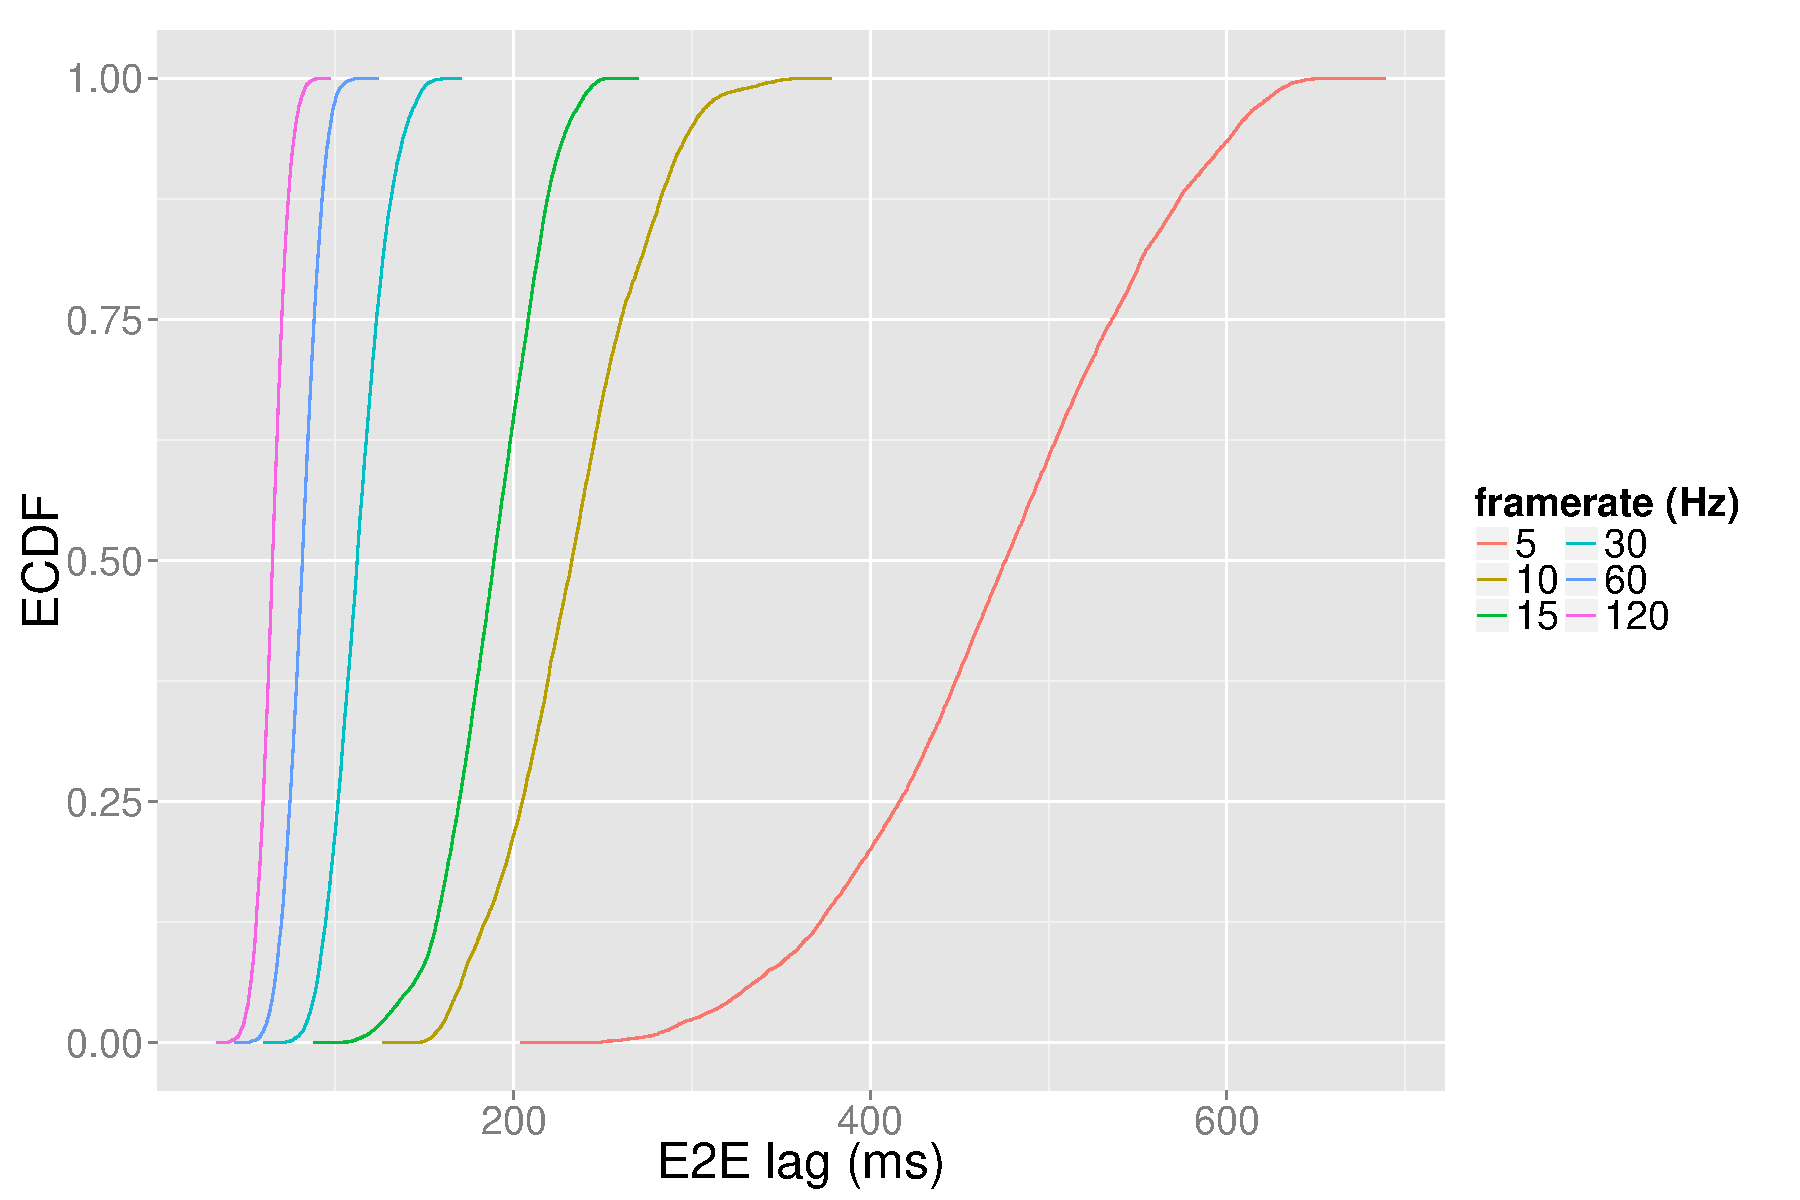
\includegraphics[width=1.0\columnwidth]{../../simulation/visualization/cloudgaming-lag-cdf.pdf}
	\caption{\acrshort{ECDF} of the influence of the rendering and streaming framerate on the end-to-end lag in the cloud scenario. Vertical intercept denotes the average base delay of \SI{68}{\milli\second}.}
	%\hoss{On average, a network delay of $\unit[2\cdot20=40]{ms}$ (correct???) exists. A constant encoding time (\unit[15]{ms}) and decoding time (\unit[5]{ms}) is assumed. Thus, the major part of the e2e lag is caused by the framerate setting. Kann man hier noch eine Linie reinzeichnen, die die Summe 5+15+40=60 ms zeigt?}}
	%
	% Albert: Uh, oh, the cloud simulation seems to have reused a stray 
	%         200 Hz setting for $c$ from a previous online game sim.
	%         I'm documenting that this value has been used.
	%
\label{fig:cloud-e2e-delay-sim}
\end{figure}

Figure~\ref{fig:cloud-e2e-delay-sim} shows the results of this scenario as an \gls{ECDF} of the end-to-end lag for several framerates. As before, the framerate impacts the end-to-end lag more severely than the network delay.
%the large influence of the framerate when compared to the network delay is evident. 
This result is of particular importance considering how past studies have relied on similarly low framerates as $5-\SI{15}{\hertz}$ when assessing the network influence on cloud gaming. Similarly, these results can provide guidelines for implementors of cloud gaming to factor in the framerate in their calculations accordingly.



%%%%%%%%%%%%%%%%%%%%%%%%%%%%%%%%%%%%%%%%%%%%%%%%%%%%%%%%%%%%%%%%%%%%%%%%%%%%%%%%
\subsection{Representative Games for QoE studies}
\label{sec:game-criteria}
%\hoss{Ich glaube der Titel triffts noch nicht so ganz. Choosing Representative Games for QoE Studies? }
The three scenarios presented here serve to provide initial insights into the complex interactions of the end-to-end lag. Although the underlying abstract model adopts some simplifications and some properties are not factored in yet, the results are still very revealing. Using the model and simulator as baseline, one can get a good estimation of the expected video game \gls{QoS} values. Alternatively, it can help in choosing representative games for select scenarios.


The result of any game quality assessment strongly depends on the considered game, as each game is a unique collection of individual game mechanics, each bringing a distinct influence onto the assessment alongside with it. Here we provide a foundation for quality metrics by rather investigating game-independent metrics, including the framerate, frame \gls{IAT}, and the end-to-end lag.


%%%%%%%%%%%%%%%%%%%%%%%%%%%%%%%%%%%%%%%%%%%%%%%%%%%%%%%%%%%%%%%%%%%%%%%%%%%%%%%%
\subsubsection{Game Independent Metrics}
%\hoss{Was soll hier gesagt werden? Selecting the right parameter range for framerate?}
Framerate and frame \gls{IAT} are a good indicators for the game's fluidity and responsiveness to inputs. As such, choosing the right range for these parameters is especially important in cloud gaming scenarios or for quality assessments. End-to-end lag gives the best overall picture on the attainable gaming experience and should always be preferred over partial lag values, e.g. by purely investigating the network latency. The impact of the lag also depends on the type and precision of controls the game offers. For example, a keyboard and mouse driven PC game might be much more sensitive to high lag values than a mobile game with touch controls.

Input controls are but one aspect of the games environment and settings, which need to be carefully selected to achieve meaningful results. This especially concerns PC games which usually offer a wide range of options to choose from. Here, the graphics options are the most impactful. The recommended settings to run games at are a video resolution of 1080p or higher with the games other graphics options set to high or at least medium values in order to reflect a typical gaming experience. Due to the demonstrated impact of the framerate on the end-to-end lag a target of \SI{60}{\hertz} should considered as a minimum rate for most games. Some types of games are less dependent on the framerate, where a rate of \SI{30}{\hertz} would still be considered acceptable.

% Experimenters should never set a framerate lower than that for the reasons discussed in the previous section. They should however also consider testing at higher framerates, especially for competitive games with a high tickrate to further reduce the negative impact of low framerates.

%The general focus here lies on measuring online games with high demands. The idea is that if these games work at an objectively good quality, it is reasonable to assume that all other games do so as well.


%%%%%%%%%%%%%%%%%%%%%%%%%%%%%%%%%%%%%%%%%%%%%%%%%%%%%%%%%%%%%%%%%%%%%%%%%%%%%%%%
\subsubsection{Quantifiable Game Classification Criteria}

Finding games which are representative for certain input and lag demands is challenging. For example, the traditional game genre categorization is not a good starting point, as games from the same category can be vastly different in terms of game speed and necessary reaction times. Rather, the following four exemplary metrics might prove useful when classifying games to better assess the impact of the end-to-end lag on the experienced quality.

\textbf{Required number of decisions or actions in a certain time span} E.g., the \gls{CCG} \textsc{Hearthstone} may only require a handful of actions, i.e. choosing and playing cards, each turn, while in order to competitively play the \gls{RTS} \textsc{Starcraft 2} you more or less need to achieve a few hundred \gls{APM}, with the record being higher than $800$ \gls{APM}. \cite{6404025} defines a related metric dubbed \textit{command heaviness} comparing the amount of change to the input rate, under the umbrella term \textit{real-time strictness}. Micromanagement-intense games usually tend to result in high APM rates.

\textbf{Maximum successful reaction time to in-game actions} Again e.g., \textsc{Hearthstone} as a turn-based game requires no instant reaction time at all, as the opponent's and the player's actions are separated into turns. First-person shooters like \textsc{Counter-Strike: Global Offensive} are usually on the opposite extreme of this spectrum, as they tend to have a very high tickrate and literally often require you to ``shoot first'' to win. This is also investigated in \cite{Claypool:2006:LPA:1167838.1167860}.

\textbf{Ratio of unpredictable actions} This is closely related to the previous metric. When considering an entirely rhythm-based game (e.g., \textsc{Guitar Hero}), where you can completely pre-plan all of your actions, to a twitch-based shooter like \textsc{Counter-Strike} where you have to react from moment to moment. In theory, a game with no surprising events will be less influenced by a higher end-to-end lag.

\textbf{Temporal and spatial accuracy and precision of input events} Accuracy can be relevant in both temporal as well as spatial aspects. Thus, it can be influenced by both the image quality and the frame rate. For example, discrete events, e.g., button-presses on a controller, require less spatial precision than analogue inputs, e.g., free-form mouse movement.

This is a non-exhaustive list of selected quantifiable criteria. It should be refined in future studies and extended before such metrics can be applied as a means of categorization. Moreover, the value of some of these metrics might not be that easy to determine as they involve playing the game. Even as a qualitative discriminator or when considering broad value ranges, such a classification might be much more sensible than one purely based on the video game genre.

% Ultimately, to capture any and all latency sources in gaming you would need to rely on external recording gear.
% With modified input: zero latency and visible input detection (e.g. solder some LEDs to the buttons)

% Also Arduino with photodiode method described in \cite{beyermethod}
% Both this and camera method also work for closed game consoles


%%%%%%%%%%%%%%%%%%%%%%%%%%%%%%%%%%%%%%%%%%%%%%%%%%%%%%%%%%%%%%%%%%%%%%%%%%%%%%%%
%\subsection{Evaluated Metrics}

%%%%
%\subsubsection{Frame Rates and Frame Times (i.e. frame IAT)}
%i.e. frame IAT
%Reasoning for frame IAT and the negligence of past investigations
%%%%
%\subsubsection{Total and additional end-to-end latency}
%physical controller input to in-game reaction
%different in-game actions have already difference in latency, therefore need to test various actions for a complete picture
%Also discuss RTT as Hz (1/RTT) as measure for interactivity


%%%%%%%%%%%%%%%%%%%%%%%%%%%%%%%%%%%%%%%%%%%%%%%%%%%%%%%%%%%%%%%%%%%%%%%%%%%%%%%%
%\subsection{Reasonable Configuration/Setting Ranges to Test}

% Resolution: Minimum 720p, 1080p recommended, even higher is better (1440p or 2160p)
% Frame rate: 60 fps very much recommended, 30 absolute minimum,  120 or 144 can also be feasible
% Configure games to run at high or at least medium settings
% For console games: use the games intended settings for the console, never downscale the game or reduce the frame rate for streaming
% Assume no network latency higher than 200ms, preferably less than 100ms
% Assume typical access link conditions, i.e. no less than 10-16Mb/s



%Works only for general purpose computing devices with full access.
%Easiest method, but might not capture full end-to-end latency.
%FRAPS, OBS, DirectX Hooking, MSI Afterburner
%FCAT as hybrid solution with external capture card and computer


% \url{http://www.red.com/learn/red-101/high-frame-rate-video}


% articles:
% why frametimes
%     \url{https://techreport.com/review/21516/inside-the-second-a-new-look-at-game-benchmarking}

% Inside the second with Nvidia's frame capture tools
%     \url{https://techreport.com/review/24553/inside-the-second-with-nvidia-frame-capture-tools}

 % As the second turns: the web digests our game testing methods
 %    \url{https://techreport.com/blog/24133/as-the-second-turns-the-web-digests-our-game-testing-methods}

% GPU Reviews: Why Frame Time Analysis is important
%     \url{http://www.vortez.net/articles_pages/frame_time_analysis.html}

% Durante's Witcher 3 analysis: the alchemy of smoothness
%     \url{http://www.pcgamer.com//durantes-witcher-3-analysis-the-alchemy-of-smoothness/}


% Analysing Stutter – Mining More from Percentiles
%     \url{https://developer.nvidia.com/content/analysing-stutter-%E2%80%93-mining-more-percentiles-0}

% fraps vs fcat method
%     \url{http://www.extremetech.com/gaming/154089-after-almost-20-years-gpu-benchmarking-is-moving-past-frames-per-second}

% FRAPS + FRAFS
% \url{http://www.fraps.com/}
% \url{http://sourceforge.net/projects/frafsbenchview/}
% \url{http://www.5group.com/wordpress/2012/07/14/gpu-mist-pre-release-1-0-rc1/}

% issue: Fraps measures the flip queue input rather then the actual render output frames which is fine when measuring FPS but is rather poor if you want to measures actual frame times and analyze microstutter.


% NVIDIA FCAT
% \url{http://www.geforce.com/hardware/technology/fcat}
% \url{http://www.overclockers.com/nvidias-fcat-gpu-testing-pursuing/}


% Valve for Linux GL Games
% \url{https://github.com/ValveSoftware/voglperf}

% Info über MSI Afterburner overlay? oder GF experience? GPU-Z? Rivatuner Statistics Server?
% \url{http://www.overclock.net/a/how-to-use-rivatuner-afterburner-on-screen-display-and-more}



% \url{https://en.wikipedia.org/wiki/Game_classification}
% \url{https://en.wikipedia.org/wiki/Video_game_genre}
% \url{https://en.wikipedia.org/wiki/List_of_video_game_genres}


%!TEX root = paper.tex
%%%%%%%%%%%%%%%%%%%%%%%%%%%%%%%%%%%%%%%%%%%%%%%%%%%%%%%%%%%%%%%%%%%%%%%%%%%%%%%%
\section{Representative Games for QoE studies}
\label{sec:game-criteria}
%\hoss{Ich glaube der Titel triffts noch nicht so ganz. Choosing Representative Games for QoE Studies? }

The result of any game quality assessment strongly depends on the considered game, as each game is a unique collection of individual game mechanics, each bringing a distinct influence onto the assessment alongside with it. Here we provide a foundation for quality metrics by rather investigating game-independent metrics, including the framerate, frame \gls{IAT}, and the end-to-end lag.


%%%%%%%%%%%%%%%%%%%%%%%%%%%%%%%%%%%%%%%%%%%%%%%%%%%%%%%%%%%%%%%%%%%%%%%%%%%%%%%%
\subsection{Game Independent Metrics}
%\hoss{Was soll hier gesagt werden? Selecting the right parameter range for framerate?}
Framerate and frame \gls{IAT} are a good indicators for the game's fluidity and responsiveness to inputs. As such, choosing the right range for these parameters is especially important in cloud gaming scenarios or for quality assessments. End-to-end lag gives the best overall picture on the attainable gaming experience and should always be preferred over partial lag values, e.g. by purely investigating the network latency. The impact of the lag also depends on the type and precision of controls the game offers. For example, a keyboard and mouse driven PC game might be much more sensitive to high lag values than a mobile game with touch controls.

Input controls are but one aspect of the games environment and settings, which need to be carefully selected to achieve meaningful results. This especially concerns PC games which usually offer a wide range of options to choose from. Here, the graphics options are the most impactful. The recommended settings to run games at are a video resolution of 1080p or higher with the games other graphics options set to high or at least medium values in order to reflect a typical gaming experience. Due to the demonstrated impact of the framerate on the end-to-end lag a target of \SI{60}{\hertz} should considered as a minimum rate for most games. Some types of games are less dependent on the framerate, where a rate of \SI{30}{\hertz} would still be considered acceptable.

% Experimenters should never set a framerate lower than that for the reasons discussed in the previous section. They should however also consider testing at higher framerates, especially for competitive games with a high tickrate to further reduce the negative impact of low framerates.

%The general focus here lies on measuring online games with high demands. The idea is that if these games work at an objectively good quality, it is reasonable to assume that all other games do so as well.


%%%%%%%%%%%%%%%%%%%%%%%%%%%%%%%%%%%%%%%%%%%%%%%%%%%%%%%%%%%%%%%%%%%%%%%%%%%%%%%%
\subsection{Quantifiable Game Classification Criteria}

Finding games which are representative for certain input and lag demands is challenging. For example, the traditional game genre categorization is not a good starting point, as games from the same category can be vastly different in terms of game speed and necessary reaction times. Rather, the following four exemplary metrics might prove useful when classifying games to better assess the impact of the end-to-end lag on the experienced quality.

\myparagraph{Required number of decisions or actions in a certain time span} E.g., the \gls{CCG} \textsc{Hearthstone} may only require a handful of actions, i.e. choosing and playing cards, each turn, while in order to competitively play the \gls{RTS} \textsc{Starcraft 2} you more or less need to achieve a few hundred \gls{APM}, with the record being higher than $800$ \gls{APM}. \cite{6404025} defines a related metric dubbed \textit{command heaviness} comparing the amount of change to the input rate, under the umbrella term \textit{real-time strictness}. Micromanagement-intense games usually tend to result in high APM rates.

\myparagraph{Maximum successful reaction time to in-game actions} Again e.g., \textsc{Hearthstone} as a turn-based game requires no instant reaction time at all, as the opponent's and the player's actions are separated into turns. First-person shooters like \textsc{Counter-Strike: Global Offensive} are usually on the opposite extreme of this spectrum, as they tend to have a very high tickrate and literally often require you to ``shoot first'' to win. This is also investigated in \cite{Claypool:2006:LPA:1167838.1167860}.

\myparagraph{Ratio of unpredictable actions} This is closely related to the previous metric. When considering an entirely rhythm-based game (e.g., \textsc{Guitar Hero}), where you can completely pre-plan all of your actions, to a twitch-based shooter like \textsc{Counter-Strike} where you have to react from moment to moment. In theory, a game with no surprising events will be less influenced by a higher end-to-end lag.

\myparagraph{Temporal and spatial accuracy and precision of input events} Accuracy can be relevant in both temporal as well as spatial aspects. Thus, it can be influenced by both the image quality and the frame rate. For example, discrete events, e.g., button-presses on a controller, require less spatial precision than analogue inputs, e.g., free-form mouse movement.

This is a non-exhaustive list of selected quantifiable criteria. It should be refined in future studies and extended before such metrics can be applied as a means of categorization. Moreover, the value of some of these metrics might not be that easy to determine as they involve playing the game. Even as a qualitative discriminator or when considering broad value ranges, such a classification might be much more sensible than one purely based on the video game genre.
%!TEX root = paper.tex
%%%%%%%%%%%%%%%%%%%%%%%%%%%%%%%%%%%%%%%%%%%%%%%%%%%%%%%%%%%%%%%%%%%%%%%%%%%%%%%%
\section{Conclusion}
\label{sec:conclusion}

%These scenarios reveal the necessity of a tight control over game parameters, such as the framerate, resolution, or input devices, in accordance with the game's type.

This paper presents a model for \acrfull{E2E} lag in video games, including online and cloud variants. The \gls{E2E} lag represents the time elapsed between a player input event such as mouse movement or keystrokes and the display of the event's results in the game on the local display. This lag is a main governing factor for \acrfull{QoE} in human-computer interaction in general, and video games in particular. The model is parameterized on the command rate at which batched user events are processed, the server tickrate and state processing time, the game's local framerate, the network delay (for online games), and codec delays (for cloud games). % Note: We don't look at local latencies really: Mice and keyboards, USB, TV sets, multibuffering, ...
The model is simulated using \acrfull{DES}, showing the dominant influence of the game framerate on the \gls{E2E} lag particularly for low framerates. This contribution to \gls{E2E} lag may even mask the influence of network delay, yet it appears underrepresented in previous work.  On an abstracted level, the model helps to explain the mechanics behind lag in different game types and architectures. This is of interest to both actual implementations of games and study design for game \gls{QoE} assessment. To foster participation, the model simulation code used for this paper is available as free, open-source software from the authors' repository~\cite{onlinegame-lag-sim-repo}, as are the raw data.
%
%results, meta: explains lag mechanics, helps judge correctness of qoe models
%results, numbers: parameter study for local, online, cloud games.
%
%fuwo: use this to make better studies
%
%
%, , is an important influence 
%The \acrfull{QoE} of depends partially on the lag 
%The models presented here serve to provide initial insights into the complex interactions of \gls{E2E} game lag. Although the underlying abstract model adopts some simplifications and some properties are not incorporated yet, the results are still very revealing. Using the model and simulator as baseline, one can get a good estimation of the expected video game \gls{QoS} values. 
%%Alternatively, it can help in choosing representative games for select scenarios.
%A proper setup of gaming \gls{QoS}/\gls{QoE} studies is of critical importance to their validity. The \gls{E2E} lag queuing model set up in this work can support these endeavors a long way through an improved understanding of relevant game properties and their interactions. The role of the framerate, and its lag-inducing effects has been undervalued in the past, which these models and simulations aim to rectify. Of special interest is the masking effect low values of the framerate or tickrate have on the network delay on the \gls{E2E} lag. This and similar side effect need to be considered for subsequent research efforts.

\eightpt
\printbibliography[title={References}, heading=bibnumbered]


\end{document}
